\documentclass[11pt,a4paper,twoside,openright]{report}

\usepackage[dvips]{graphicx}
\usepackage{tabularx}
\usepackage{afterpage}
\usepackage{amsmath,amssymb}
\usepackage{bm}
\usepackage{mathtools}
\usepackage{rotating}
\usepackage{fancyhdr}
\usepackage{lipsum}
\usepackage[scriptsize]{caption}
% \usepackage{subcaption}
% \usepackage{algpseudocode}
\usepackage{algorithm}
\usepackage{subfig}
% \usepackage{tikz}
% \usepackage{pgfplots}
% \usepgfplotslibrary{fillbetween}
% \pgfplotsset{compat=1.14}
% \allowdisplaybreaks
\usepackage{algorithmic}
\usepackage{hyperref}
\usepackage[space]{grffile} % to use space in the file path
\usepackage{color}
\usepackage[usenames,dvipsnames]{pstricks}
\usepackage{epsfig}
\usepackage[usenames,dvipsnames]{pstricks}
\usepackage{epsfig}
\usepackage{pst-grad} % For gradients
\usepackage{pst-plot} % For axes
\usepackage[space]{grffile} % For spaces in paths
\usepackage{etoolbox} % For spaces in paths
\makeatletter % For spaces in paths
\patchcmd\Gread@eps{\@inputcheck#1 }{\@inputcheck"#1"\relax}{}{}
\makeatother
% User Packages:
\usepackage{amssymb,amsthm,amsmath}
\usepackage{mathtext}
\usepackage{amsthm}
% \usepackage[algcompatible]{algpseudocode}

\usepackage{placeins}
% To ensure figure to be in the correct subsection
%\usepackage{placeins}
%
%\let\Oldsection\section
%\renewcommand{\section}{\FloatBarrier\Oldsection}
%
%\let\Oldsubsection\subsection
%\renewcommand{\subsection}{\FloatBarrier\Oldsubsection}
%
%\let\Oldsubsubsection\subsubsection
%\renewcommand{\subsubsection}{\FloatBarrier\Oldsubsubsection}
\hyphenation{con-fi-gu-ra-zio-ne}

\setlength{\oddsidemargin} {2. cm}
\setlength{\evensidemargin} {2. cm}
\addtolength{\oddsidemargin} {-0.4 cm}
\addtolength{\evensidemargin} {-0.4 cm}
\linespread{1.1}

\usepackage[english]{babel}
\usepackage[nottoc]{tocbibind}
% \usepackage[latin1]{inputenc}
\renewcommand{\captionfont}{\normalfont \sffamily \itshape \small}
\captionsetup[algorithm]{justification = raggedright, singlelinecheck = false}

\pagestyle{empty}

\newtheorem{definition}{Definition}[section]
\newtheorem{theorem}{Theorem}[section]
\newtheorem{corollary}{Corollary}[section]
\newtheorem{assumption}{Assumption}
\newtheorem{lemma}{Lemma}[section]
\usepackage[draft]{todonotes}
\DeclareMathOperator*{\argmin}{arg\,min}
\DeclareMathOperator*{\arginf}{arg\,inf}

\begin{document}
\thispagestyle{empty}
\vspace*{-1.5cm}
 \bfseries{
\begin{center}
  \large
  POLITECNICO DI MILANO\\
  \normalsize
  Mathematical Eng Master Degree\\
  Dipartimento di Mate\\
  \begin{figure}[htbp]
    \begin{center}
      %\includegraphics[width=3.5cm]{./img/logo/logo poli}
      
\includegraphics[width=5cm]{./img/logo/digi3.png}
    \end{center}
  \end{figure}
  \vspace*{0.1cm} \LARGE


    \textbf{Il Grinch Aveva Ragione}\\


  \vspace*{.75truecm} \large
 %  \vspace*{0.5truecm} \large
  Artificial Intelligence and Robotic Laboratory \newline of Politecnico di Milano
\end{center}
\vspace*{2.0cm} \large
%\vspace*{2.0cm} \large
\begin{flushleft}


  Supervisor: Prof. Marcello Restelli \\

  \begin{tabbing}  
      Co-supervisors: \=  Francesco Trov\a`{o} Ph.D.,
      Edoardo Vittori,
  \end{tabbing}
\end{flushleft}
\vspace*{1.0cm}
%\vspace*{0.5cm}
\begin{flushright}


  Master thesis of:\\ Martino Bernasconi de Luca, $\pi$\\


\end{flushright}
\vspace*{0.8cm}
\begin{center}

  Academic Year 2018-2019 % check
\end{center} \clearpage
}

\thispagestyle{empty} \normalfont \cleardoublepage
\thispagestyle{empty}  \cleardoublepage
\pagenumbering{Roman}
\begin{abstract}
Outperforming the markets through active investment strategies is one of the main challenges in finance.
The random movements of assets and the unpredictability of catalysts make it hard to perform better than the average market, therefore, in such a competitive environment, the methods designed to keep low transaction costs have a significant impact on the obtained wealth.
This thesis focuses on investing techniques to beat market returns through Online Portfolio Optimization while controlling transaction costs.
Such a framework differs from classical approaches as it assumes that the market has an adversarial behavior and no statistical characterization is enforced, requiring frequent rebalancing of the portfolio.
Within this context, most of the existing algorithms neglect transaction costs; we show that the one which provides bounded costs make unrealistic assumptions.
To deal with transaction costs, in the Online Portfolio Optimization setting, we propose the use of the Online Gradient Descent algorithm. We show that it has regret, considering costs, of the order $\mathcal{O}(\sqrt{T})$, $T$ being the investment horizon, and has $\Theta(N)$ per-step computational complexity, $N$ being the number of assets.
Furthermore, we show that this algorithm provides competitive gains when compared empirically with state-of-the-art online learning algorithms on real-world datasets.
\end{abstract}
\begin{abstract}
Una delle sfide più importanti in finanza è quella di avere prestazioni migliori rispetto ad un approccio passivo agli investimenti. I movimenti casuali del mercato e la difficoltà nel predirne i catalizzatori rendono molto ostico surclassare il mercato, e quindi, in un ambito tanto arduo, tecniche progettate per tenere bassi i costi di transazione possono avere un impatto significativo sul guadagno finale. Questa tesi si concentra su tecniche di investimento basate su \emph{Online Portfolio Optimization} controllando i costi di transazione. Questo ambito si differenzia dal classico approccio poiché assume che i mercati abbiano un comportamento avversario, senza nessuna caratteristica stocastica, il che richiede quindi che tali tecniche ridistribuiscano di frequente il loro portfolio. Molti degli algoritmi in questo ambito non considerano i costi di transazione; mostreremo che quelli che hanno un bound sui costi lo fanno con assunzioni irrealistiche. Si propone l'uso di \emph{Online Gradient Descent} per trattare il problema dei costi di transazione in Online Portfolio Optimization. Mostreremo che questo assicura un bound sul guadagno, con costi, dell'ordine di $\mathcal O(\sqrt T)$, dove $T$ è l'orizzonte temporale. Inoltre mostreremo che questo algoritmo ha complessità computazionale dell'ordine di $\Theta(N)$, dove $N$ è il numero di azioni nel portfolio.
Alla fine verificheremo sperimentalmente le garanzie teoriche dell'algoritmo e che esso, quando testato su dati reali, provvede a guadagni comparabili agli altri algoritmi nello stato dell'arte.
\end{abstract}
%\thispagestyle{empty} \vspace*{.75truecm} \cleardoublepage
%\include{chapters/acknowledgements}
\thispagestyle{empty} \vspace*{.75truecm} \normalfont \cleardoublepage
\pagestyle{plain}\renewcommand{\chaptermark}[1]{\markboth{\chaptername\ \thechapter.\ #1}{}}
\renewcommand{\sectionmark}[1]{\markright{\thesection.\ #1}}
\fancyhead[LE,RO]{\bfseries\thepage}
   
\fancyhead[RE]{\bfseries\leftmark} 
\fancyhead[LO]{\bfseries\rightmark}   
\renewcommand{\headrulewidth}{0.3pt}

\setcounter{tocdepth}{3}
\setcounter{secnumdepth}{3}
\tableofcontents
\cleardoublepage

\pagenumbering{arabic}

\listoffigures
\listoftables

\clearpage
\addcontentsline{toc}{chapter}{List of Algorithms}
\listofalgorithms
% \addtocontents{lot}{\def\string\figurename{Algorithm}}

\chapter{Introduction}

Classical investment techniques for the portfolio management problem derive from the knowledge of the statistical distribution of the assets return. Then, once the statistical model has been chosen, the problem get solved by optimizing the expected value of the utility of some random variable (usually accounting for the trade-off between risk and return), that describes the value of the portfolio in some fixed time in the future. This line of thinking has been proposed and sustained by Markovitz, Samuelson, Fama ecc... %\cite{Fortune Formula}
, and it is now called Modern Portfolio Theory (MPT).

This approach is known to be very susceptible to the errors in the modelling of the random variable that model the asset return. In fact, it is known that the markets have a non stationary behaviour, which means that every statistical assumption is ephemeral and unreliable. %\cite{qualcuno} 
and they are usually referred to to backward looking, i.e. that they optimize 

A different approach has been originated from the fields of information theory at the Bell Labs in the 1950, from the works of Shannon, Kelly and Cover. This methods were first included in the classical portfolio theory framework, under the name of Capital Growth Theory (CGT) \cite{hakansson1995capital} and then got included in the machine learning literature under the framework of Online Game Playing. Only recently this field has been taken into the Online Optimization This formulation has very interesting properties such as stability in a game theory fashion (equilibrium) and robustness versus adversarial manipulation.

One of the strongest points in favor of this techniques are the strong theoretical guarantees that algorithms developed under this framework can give. This guarantees come from the game theory concept of Regret, which is a form of dissatisfaction originated from having taken an action, instead of another action.

Principal in this thesis will be the extension of the modelling of the financial applications of this methodologies to the presence of transaction costs and to provide strong theoretical assurance even in the presence of transaction costs. In fact in many financial situations, transaction costs are not modelled and 

3\chapter{Online Learning}\label{ch:OnlineLearning}
Online Learning is a theoretical framework to formalize a sequential decision problem in which an agent has to take consecutive actions in an environment. Every time the agent takes an action, the environment returns a loss signal (or reward depending on the convention on the sign). This framework is similar to other sequential decision problems such as Reinforcement Learning \cite{sutton1998introduction}, with the exception that the loss function is decided by an adversary which has complete knowledge of your strategy in advance, rather that be described by a stochastic probability kernel. \todo{Francesco dice che è sbagliato.}
The purpose of this section is to present the general framework of Online Game Playing and to introduce the notation necessary for the development of the theory. We will define formally the framework of Online Learning with Expert Advice, which is one the most studied framework of Online Learning, due to its ability to include many other frameworks, such as Multi Armed Bandit\todo{define} or Online Convex Optimization. \todo{maybe add DAgger}
Then we will present the concept of \emph{regret} and present the relationship of Online Learning to classical repeated games, a classical framework coming from the field of Game Theory. Modern finance \todo{manca coeasion OL->finance} has more and more the need for a Game Theoretic approach, this is evident when one looks at the field of on venue market making, that can be modeled naturally as a repeated game, or in merger and acquisition that can be modeled as a normal form game. \todo{add ref e aggiustare}
Finally we will introduce Online Convex Optimization as a special case of Online Learning with expert advice and its interesting relationship to theoretical statistical learning. The choice of this path, from Online Learning to Online Convex Optimization, has been done to show how general and powerful Online Learning is in its simplicity, and why Online Convex Optimization is the most suitable framework to present our contribution to Online Portfolio Selection, that will be presented in later chapters.\todo{ref  chapter ...}

In fact, even if we will focus on the portfolio problem, the apparently simple formulation of this framework is capable to encompass many other applications and problems, such as network routing~\cite{belmega2018online} and dark pool order allocation~\cite{agarwal2010optimal}. 
A thorough dissertation of the techniques that have been developed in the field of Online Learning can be found in \cite{cesa2006prediction}.
%Cita qualcuno he dia esposizione completa

\section{Online Learning}
\label{sec:OnlineLearning}
\begin{definition}(Online Game Playing).\label{def:OGP}
    Let $\mathcal Y$ be the outcome space, $\mathcal D$ the prediction space and $f:\mathcal D\times\mathcal Y\to \mathbb R$ is a loss function, an Online Game is the following sequential game played by the forecaster $\mathcal A$ and the environment:

    For each round $t\in 1,2,\ldots$
    \begin{enumerate}
        %\item Each expert $E_i\in\mathcal E$ choose its prediction $x_{t,E_i}\in\mathcal D$
        \item The learner $\mathcal A$ chooses an element of the decision space $x_t\in\mathcal D$.
        \item The environment chooses the element $y_t\in\mathcal Y$, and subsequently determines the loss function $f(\cdot,y_t)$.
        \item The agent $\mathcal A$ incurs in a loss $f(x_t,y_t)$.
		\item The agent updates its cumulative losses $L_t=L_{t-1}+f(x_t,y_t)$ with $L_0=0$
    \end{enumerate}
\end{definition}

In Online Learning an agent $\mathcal A$ has to guess the outcome $y_t$ based on a the past outcomes $y_1,y_2,\ldots,y_{t-1}$ of some events that are in the outcome space $\mathcal Y$, at each time step she will play (sometimes we will also say \emph{predict}) $x_t$, that is an element of the prediction space $\mathcal D$, and the environment will choose a loss function $f(\cdot,y_t)$ by determining the outcome $y_t$.
Sometimes it is not important to know the exact outcome of the round and so we can identify the function $f(x,y_t)$ with $f_t(x)$. The agent $\mathcal A$ is essentially the identification of the functions that maps the history of past outcomes to the new prediction:
$$\mathcal A\equiv\left\{h_{t-1}:=(y_1,\ldots,y_{t-1})\longmapsto x_t\right\}_{t\ge 1} $$
The simplest case is for $\mathcal Y=\mathcal D$ and both of finite cardinality, meaning that there are only a finite number of actions that the agent $\mathcal A$ can choose from. 
We will sometimes refer to the environment defined in Section \ref{def:OGP} as "adversarial", since no stochastic characterization is given to the outcome sequence $y_t$ and the analysis of the regret is done assuming a worst case scenario.
Since the adversary knows the prediction $x_t$, before deciding the outcome $y_t$, absolute minimization \todo{???} of the loss is an hopeless task and so we have to set an easier task. We will also present the counterexample to why the absolute minimization of the loss is an hopeless task, and present the adapt minimal framework to successful Online Learning in Adversarial Environment.

% ==================================================

% The assumption\todo{Non qui} of a model for the data even existing is basically assuming the stationarity of the observed events. This may be reasonable in some cases, like speech recognition in which we can assume that there is constant model which translate sound of speech into its lexical transliteration, but it not as reasonable in other cases, as trivial as spam filtering. In email classification for spam filtering, the spam writers actually adapts to the filter itself and every constant model would eventually be out of fashion after some time. In such a regime you need a way of adapting your hypotheses during the learning procedure. This is were Online Learning comes to help. In Online Learning we do not make any assumption on the structure of the data and constantly adapting our hypothesis in order to asymptotically perform as the best hypothesis in hindsight.

% =================================================

\subsection{Regret and Experts}
\begin{figure}[t!]
\centering
\begin{pspicture}(0,-3.42)(8.18,3.42)
\psframe[linecolor=black, linewidth=0.04, dimen=outer, framearc=0.1](6.54,0.9)(2.78,-0.36)
\psframe[linecolor=black, linewidth=0.04, dimen=outer, framearc=0.1](6.52,3.42)(2.82,2.3)
\rput[bl](3.76,2.7){Agent: $\mathcal A$}
\rput[bl](3.68,0.12){Environment}
\psline[linecolor=black, linewidth=0.036, arrowsize=0.05291667cm 2.0,arrowlength=1.4,arrowinset=0.0]{->}(6.54,2.8)(7.66,2.8)(7.66,0.2)(6.54,0.22)
\rput[bl](7.9,1.44){$x_t$}
\psline[linecolor=black, linewidth=0.036, arrowsize=0.05291667cm 2.0,arrowlength=1.4,arrowinset=0.0]{->}(2.78,0.3)(1.46,0.3)(1.46,2.88)(2.8267796,2.8677726)
\rput[bl](0.0,1.2){$f(x_t,y_t)$}
\psframe[linecolor=black, linewidth=0.036, dimen=outer, framearc=0.1](6.2,-2.2)(3.16,-3.42)
\rput[bl](3.78,-2.92){Experts: $\mathcal E$}
\rput[bl](2.96,-1.36){$x_{e,t}$}
\rput[bl](5.26,-1.34){$f(x_{e,t},y_t)$}
\psline[linecolor=black, linewidth=0.036, arrowsize=0.05291667cm 2.0,arrowlength=1.4,arrowinset=0.0]{->}(3.8,-2.22)(3.8,-0.36)
\psline[linecolor=black, linewidth=0.036, arrowsize=0.05291667cm 2.0,arrowlength=1.4,arrowinset=0.0]{->}(5.18,-0.4)(5.18,-2.22)
\end{pspicture}

\caption{Online Learning with Expert Advice as Multi Agent-Environment interaction.}
\label{fig:OL}
\end{figure}
We stated that the objective of absolute loss minimization is hopeless in an adversarial framework, as the adversary can always choose the outcome $y_t$ that maximizes the loss $f(x,y_t)$ regardless of the decision $x\in\mathcal D$ taken by the learner. We shall present a simple counterexample in this setting.

Take $\mathcal D$ as a space of binary outcomes, \emph{i.e.} $|\mathcal D|=2$ absolute loss as $f(x,y)=|x - y|$. Since the adversary plays after the learner $\mathcal A$, it can  make the loss of the learner $L_T=T$ by outputting the bit non predicted by the learner. Notice that no assumption has been made on the strategy followed by the learner $\mathcal A$.
From this example it is clear that the learner has to set a less ambitious goal.

We do so by extending the theoretical formulation in Section \ref{sec:OnlineLearning} by including a set $\mathcal E$ of other players, this setting is called "prediction with expert advice". At each time step of the prediction game, each expert $e\in\mathcal E$, predicts an element $x_{t,e}\in\mathcal D$, and incurs in a loss $f(x_{t,e},y_t)$, just as the agent $\mathcal A$, creating a general multi-agent interaction as in Figure~\ref{fig:OL}. \todo{Spiegare figure: Non l'ho già fatto?}
Now the goal that the learner sets itself to solve is to obtain small losses with respect to the best expert in the class $\mathcal E$. This concept is captured by the definition of regret.
Formally, we define the regret $R_{T,e}$ for the agent $\mathcal A$ with respect to expert $e\in\mathcal E$ (assumed finite for the moment) as follows:

\begin{equation}\label{def:Regret}
	R_{T,e} = L_T-L_{T,e}
\end{equation}

The regret observed by the agent $\mathcal A$ with respect to the entire class of experts $\mathcal E$ is defined as:

\begin{equation}
	R_T=\max\limits_{e\in\mathcal E}R_{T,e}=L_T-\min\limits_{e\in\mathcal E}L_{T,e}.
\end{equation}

The task the agent $\mathcal A$ is set to solve is to find a sequence $x_t$ function of the information obtained up to the time $t$ in order to obtain small regret $y_T$ with respect to any sequence $y_1,y_2,\ldots$ chose by the environment.

In particular we aim to achieve sub-linear regret $y_T= o(T)$, meaning that the per-round regret $y_T/T$ will asymptotically vanish: 

\begin{equation}
	y_T= o(T) \implies \lim\limits_{T\to \infty}\frac{y_T}{T}=0,
\end{equation}

where $ o(T)$ is the space of sub-linear affine functions. A strategy $\mathcal A$ that attains sub-linear regret is called \emph{Hannan-Consistent}~\cite{hannan1957approximation}.

The regret is a measure of the distance between our online performance and the best offline (in retrospect) performance among the expert class $\mathcal E$, this is also called \emph{external regret} since it is compared to the external set of experts $\mathcal E$. A surprising fact is even that such algorithms do even exist.
Indeed a first result is that in general there are no Hannan Consistent strategies, and just introducing the concept of regret is not enough for successful Online Learning: 

A first simple counterexample can be found in~\cite{cover1966behavior}. If the decision space $\mathcal D$ is finite then there exists a sequence of loss function such that $R_T=\Omega(T)$.
% Cover Impossibility
Again take $\mathcal D$ as a space of binary outcomes, absolute loss as $f(x,y)=|x - y|$, and the class of experts is composed by two experts, one predicting always $0$ and the other always $1$. Taking $T$ odd, we have that the loss of the best expert is $L_{T,e}<\frac{T}{2}$, and we have already shown that the adversary can make the loss of the learner $L_T=T$. It is now evident that the regret is $R_T>T-\frac{T}{2}$, which do not allow $R_T/T\to 0$. This argument is easily extended in the case of any finite decision space $\mathcal D$.

In order for the learner to achieve sub-linear regret is to randomize its predictions, the learner, at each turn $t$, holds a probability distribution on the decision space and plays $x_t$ according to this distribution. Clearly the adversary has knowledge of the probability distribution of the learner $\mathcal A$, but has no knowledge of the random seed used by the agent $\mathcal A$, \emph{i.e.} does not know the actual decision taken according to the distribution held by the agent. If the original decision space was $\mathcal D$ with $|\mathcal D|=N$ after the randomization of the decision, we effectively transformed the decision space $\mathcal D$ into the $\Delta_{N-1}\in\mathbb R^{N}$ probability simplex. By doing so we are formally extending the game into its mixed extension, as will be discussed further in Section \ref{sec:GT}. It can be viewed also as a \emph{covexification} of the domain, pointing to the undeniably necessity of convex geometry in this context, that will be discussed in \ref{sec:OCO}. Therefore, from now on the domain $\mathcal D$ will be convex, either by the problem specification or by randomized convexification if the problem has discrete decision space.

\subsection{Existence of No-Regret Strategies}
In this section we will show the existence of Hannan-consistent strategies in the case of finite experts and provide a general form to generate sub-linear regret strategies. 
The general idea with a finite class of experts is given by the Weighted Average Forecaster. A natural class of algorithm to explore is the predicting as the weighted average prediction of the experts predictions, weighted on the accrued regret suffered by the agent $\mathcal A$:

\begin{definition}(Weighted Average Forecaster).\label{def:weighted_avg}
For a finite class of experts $\mathcal E$ the weighted average prediction is defined as
\begin{equation}
	x_t = \frac{\sum\limits_{i=1}^{N}w_{t-1,i}x_{t,i}}{\sum\limits_{i=1}^{N}w_{t-1,i}},
\end{equation}
where $w_{t-1,i}>0$ and $x_{t,i}$ is the prediction of expert $E_i\in\mathcal E$ at round $t$. 
\end{definition}

Since $\mathcal D$ is convex we have that $x_t\in\mathcal D$.
Then it is natural to assume that the weights are a function of the cumulated regret suffered by the agent with respect to the experts, and also that the change in weight is proportional to the change in a potential function:
We can generalize the simple weighted average prediction \eqref{def:weighted_avg} in the following general form, introduced in~\cite{cesa2003potential}:

\begin{equation}\label{eq:potential_avg}
x_t = \frac{\sum\limits_{i=1}^{N}\partial_i \Phi(\mathbf R_{t-1}) x_{t,i}}{\sum\limits_{i=1}^{N}\partial_i \Phi(\mathbf R_{t-1}) },
\end{equation}

where $\Phi(\mathbf u)=\varphi\left(\sum\limits_{i=1}^N\phi(u_i)\right)$ is a function $\Phi:\mathbb R^N\to\mathbb R^+$ defined through two increasing functions $\phi,\varphi:\mathbb R\to\mathbb R^+$, $\varphi,\phi\in\mathcal C^2(\mathbb R)$ and concave and convex, respectively and $\mathbf R_T=(R_{T,1},\ldots,R_{T,N})$.
By specializing the two functions $\varphi,\phi$ we can derive most of the algorithm for dealing with prediction under expert advice.
The reasons behind the general form of Equation \eqref{eq:potential_avg} and an extended discussion can be found in~\cite{hart2001general},~\cite{cesa2003potential} and~\cite{blackwell1956analog}, but the general idea is that the form of Equation \eqref{eq:potential_avg} has the following property:

\begin{theorem}
	If $x_t$ is given by Equation~\eqref{eq:potential_avg} and the loss $f(\cdot,y)$ is convex in the first argument then the instantaneous weighted regret satisfies:  
	$$\sup\limits_{y_t\in\mathcal Y}\sum\limits_{i=1}^N[f(x_t,y_t)-f(x_{t,i},y_t)]\partial_i \Phi(\mathbf y_{t-1}) \le 0$$.
\end{theorem}

\begin{proof}
	By convexity of $f(\cdot,y_t)$ we have that 
\begin{align}
	f(x_t,y_t)\le\frac{\sum\limits_{i=1}^N\partial_i\Phi(\mathbf R_{t-1})f(x_{t,i},R_t)}{\sum\limits_{i=1}^N\partial_i\Phi(\mathbf R_{t-1})}, \forall y_t\in\mathcal Y\label{eq:blw_cond}
\end{align}
And since $\Phi(\mathbf x)=\varphi\left(\sum\limits_{i=1}^N \phi(x_i)\right)$ we have that $$\partial_i\Phi(\mathbf x)=\varphi'\left(\sum\limits_{i=1}^N\phi(x_i)\right)\phi'(x_i)\ge0$$
Hence we can rearrange the terms in Equation~\eqref{eq:blw_cond} to obtain the statement.
\end{proof}

Note that fixing the structure for the weights as in Equation \eqref{eq:potential_avg} we have that $w_{t,i}\propto\phi'(R_{t,i})$ that is an increasing function in $R_{t,i}$ (since $\phi$ is convex and increasing) that essentially states that we are increasing the probability of playing actions on which we saw high regret $R_{t,i}$\todo{check}.

\begin{definition}\label{eq:ewf}
	The exponentially weighted algorithm is \eqref{eq:potential_avg} with $\varphi(x)=\frac{1}{\eta}ln(x)$ and $\phi(x)=e^{\eta x}$ giving weights of the form $w_{t-1,i}=e^{\eta y_{t-1,i}}/\sum\limits_{j=1}^Ne^{\eta y_{t-1,j}}$
\end{definition}

It can be shown \todo{e allora show} that the algorithm defined by the update rule in Equation \eqref{eq:ewf}, and for a convex loss function $f(\cdot,y_y)$, gives the following guarantee on the regret:
\begin{equation}\label{eq:regret_ewf}
R_T\le \frac{log(N)}{\eta}+\frac{T\eta}{8}\end{equation},

By choosing $\eta=O\left(\sqrt\frac{1}{T}\right)$ we obtain a sub-linear regret $R_T=\mathcal O(\sqrt T)$. %It is also possible to make this algorithm an all-time algorithm (no need to know the length of the game $T$, as opposed as a \emph{one-time} algorithm) by using the so called doubling trick by continually adapting the parameter $\eta$. In general a one-time algorithm obtains slightly smaller bounds then the all-time counterparts, that require the knowledge



\subsection{Experts}
The theoretical framework described in Section \ref{sec:OnlineLearning} is very general and most suited for a game theory analysis of the problem. This help us describe many other frameworks, such as Online Optimization, or Multi Armed Bandit (MAB) as embedded into a Game Playing framework with expert advice. It can then be specialized by fixing many elements of the definition, in order to be applied to the specific problem we are willing to solve.
For instance, the class of experts $\mathcal E$ is most of the time completely fictitious, meaning that the experts are not real players of the game, but most of the time they are \emph{simulable} meaning that the agent $\mathcal A$ is able to compute $x_{t,e}$ for each expert $e\in\mathcal E$ and most of the times the class of expert is very limited in its actions, \emph{e.g.} $\mathcal E$ is the class of experts for which $x_{t,e}$ is constant in $t$. In this case, which is the most studied class of experts, we are basically just comparing our learner $\mathcal A$ to the best fixed action $x^*$ in hindsight. This is a clairvoyant strategy that attains the minimum cumulative loss over the entire length of the game $T$.

\subsection{Uncountable Experts}\label{sec:uncountable_exp}

In the case of uncountable experts the Exponentially Averaged Prediction cannot be applied directly, but can be extended to a continuous mixture of experts predictions. More specifically we need the case of the class $\mathcal E$ being generated by a convex hull of a finite number of a base class of experts, $\mathcal E_N$.
With continuous class of experts $\mathcal E$ defined in this way, the regret definition becomes:

\begin{equation}
    R_T = \sup\limits_{q\in\Delta_{N-1}}R_{T,q}:=L_T-\inf\limits_{q\in\Delta_{N-1}}L_{T,q},
\end{equation}



where $\Delta_{N-1}\subset \mathbb R^{N}$ is the $N$-simplex, and 

$$L_{T,q}=\sum\limits_{t=1}^T f(\langle q,x_{t,e}\rangle,y_t),$$
where $x_{t,e}=(x_{t,1},\ldots,x_{t,N})\in\mathbb R^N$ is the vector of expert predictions at time $t$.
\subsection{Exp-Concave loss functions}
It will be important for the study of Portfolio Optimization the exp-concave class of loss functions.
$f(\cdot,y)$ is $\nu$-exp concave if $e^{-\nu f(\cdot,y)}$ is concave.

\begin{theorem}\label{th:General_Blk}
The Exponentially Weighted Average forecaster, for $\nu$-exp concave loss functions and for $\eta=\nu$ has the following property:

$$\Phi(\mathbf R_T)\le \Phi(\mathbf R_0)$$

where $\Phi(x)=\varphi\left(\sum\limits_{i=1}^N\phi(x_i)\right)$ is chosen as $\varphi(x)=\frac{1}{\nu}log(x)$ and $\phi(x)=e^{\nu x}$

\end{theorem}

\begin{proof}
    The weights are given by $w_{t-1,i}=e^{\nu y_{t-1,i}}/\sum\limits_{j=1}^N e^{\nu y_{t-1,j}}$.
    By exp-concavity we have that
    \begin{equation}
        e^{-\nu f(x_t,y_t)}=exp\left\{-\nu f \left(\frac{\sum\limits_{i=1}^N w_{t-1,i}x_{t,i}}{\sum\limits_{i=1}^N w_{t-1,i}},y_t\right)\right\}\ge \frac{\sum\limits_{i=1}^N w_{t-1,i}e^{-\nu f(x_{t,i},y_t)}}{\sum\limits_{i=1}^N w_{t-1,i}}
    \end{equation}
    this can be rewritten as 
    \begin{equation}\label{eq:conc_exp_last}
        \sum\limits_{i=1}^N e^{\nu y_{t-1,i}}e^{\nu [f(x_t,y_t)-f(x_{t,i},y_t)]}\le \sum\limits_{i=1}^N e^{\nu y_{t-1,i}}
    \end{equation}
    Applying $\varphi(x)=\frac{1}{\nu}log(x)$ to both sides of equation \eqref{eq:conc_exp_last} we obtain that $$\Phi(\mathbf R_{t})\le \Phi(\mathbf R_{t-1})$$ that prove the thesis.
\end{proof}

The case of exp concave functions is very special, since we can obtain Theorem~\ref{th:General_Blk} that can be used to prove regret bounds very easily:

\begin{equation}\label{eq:regret_exp_finite}
    R_T\le \frac{1}{\eta}\log\left(\sum\limits_{i=1}^N e^{\nu R_T,j}\right)=\Phi(\mathbf R_T)\le\Phi(\mathbf R_0) = \frac{log N}{\eta}
\end{equation}

The case of exp-concave losses is also useful for the case of uncountable experts sketched in Section~\ref{sec:uncountable_exp}. This formulation will be of central importance for the portfolio optimization problem.

It is natural to extend the Exponential Weighted Majority algorithm described by equation \eqref{def:weighted_avg} into its continuous case by:

\begin{equation}\label{eq:mixture}
    x_t=\frac{\int\limits_{\Delta_{N-1}} w_{q,t-1}\langle q,x_{t,e}\rangle dq}{\int\limits_{\Delta_{N-1}} w_{q,t-1}dq}
\end{equation}

\begin{theorem}(Mixture forecaster for exp-concave losses).\label{th:mixture_forecaster}
    Choosing $w_{q,t-1}=exp\left\{-\eta\sum\limits_{s=1}^{t-1}f(\langle q,x_{t,e}\rangle,y_s)\right\}$ in Equation \eqref{eq:mixture}, for a bounded $\nu$-exp concave loss function $f(\cdot,y)$, we obtain
    $$R_T\le N\nu\left(log\left(\frac{\nu T}{N}\right)+1\right)$$
\end{theorem}

Even in the case of uncountable many experts, exp-concavity of the loss function gives a better convergence rate of $\mathcal O(\log T)$then the exponentially weighted algorithm in Equation~\eqref{eq:regret_ewf}, which is $\mathcal O(\sqrt T)$.

% REGRET MINIMIZATION IN GAMES =================================================
\section{Regret Minimization in Games}
\label{sec:GT}\todo{Forse da togliere tutto questo s{}ubchpt}
In this section we explore the connection of the framework of Section \ref{sec:OnlineLearning} into a more classical repeated game framework. In the previous Section we looked at the adversary as a black box, without any specific model in mind. The reason of this chapter is to clarify its role as a player in the game and to show the game theoretical properties of Hannan-consistent agents. Since in Online Learning the convention is to speak about losses, we shall speak about losses (minimization) also in the classical definitions of game theory instead of payoffs (maximization).

\begin{definition}(Strategic Form $K$-Player Game).\label{def:Game}
    A Strategic form $K$-player game is t a tuple $\langle\mathcal K,\{X_i\}_{i\in\mathcal K},\{l_i\}_{i\in\mathcal K}\rangle$ where
    \begin{enumerate}
        \item $\mathcal K=\{1,\ldots,K\}$ is the finite set of players
        \item $X_i$ is the set of actions available to player $i\in\mathcal K$
        \item $l_i:\bigotimes\limits_{k=1}^KX_i\to\mathbb R$ is the loss observed by player $i\in\mathcal K$
    \end{enumerate}
	The game is called finite if $|X_i|<+\infty$ for all $i\in\mathcal K$.
\end{definition}


\subsection{Mixed extension}\label{sec:mixed}
As in Section~\ref{sec:OnlineLearning} we saw that it is impossible to obtains sub-linear regret in adversarial environment with finite decision space $\mathcal D$. A first step to solve this has been the \emph{randomized convexification}, where finite action spaces are extended into convex sets, given by their probability simplex, also losses are to be interpreted as expected losses when the mixed extension is applied to the formal game. More formally: 

\begin{definition}(Mixed-extension for finite games).
A finite game $\langle\mathcal K,\{X_i\}_{i\in\mathcal K},\{l_i\}_{i\in\mathcal K}\rangle$ can be extended into the game $\langle\mathcal K,\{\tilde X_i\}_{i\in\mathcal K},\{\tilde l_i\}_{i\in\mathcal K}\rangle$
\begin{enumerate}
	\item $\tilde X_i=\Delta_{|X_i|-1}\subset \mathbb R^{|X_i|}$ for all $i\in\mathcal K$ 
	\item $\tilde l:\bigotimes \tilde X_i\to\mathbb R$ is defined as
	$$\tilde l(x_1,\ldots,x_K)=\sum\limits_{i_1=1}^N\cdots\sum\limits_{i_K=1}^Np_{i_1}\ldots p_{i_K}l(i_1,\ldots,i_K)$$ 
\end{enumerate}
\end{definition}

Due to the impossibility result of Cover~\cite{cover1966behavior}, we have to work with the mixed extension formulation of the game. So from now on we take this step implicitly.
The taxonomy of game definition is quite extended and complex, we will focus on non-cooperative games \todo{cita qualcuno} since they are closely related to the setting tacked in the Online Learing field. More specifically, we will need the model for \emph{Zero Sum Game}. 

\begin{definition}($2$-Player Zero-Sum Game).\label{def:ZSG}
A Zero Sum game is a tuple $\langle\{X_1,X_2\},l:X_1\times X_2\to\mathbb R\rangle$. As in Definition~\ref{def:Game} $X_1,X_2$ are the action spaces for Player $1$ (row player) and Player 2 (columns player) respectively and $l(x_1,x_2)$ for $x_i,x_2\in X_1\times X_2$, represents the losses for Player $1$ and profits for player $2$.
\end{definition}

If this game is played for $T$ turns, we can call it a repeated game, and the losses for each player will be $L_1^{(T)}=\sum\limits_{t=1}^Tl_i\left(x_i^{(t)},x_2^{(t)}\right)$ and $L_2^{(T)}=-L_1^{(T)}$. 


\subsection{MinMax Consistency}
The question of what guarantees does Hannan-consistent strategies bring to the game theoretical formulation of the problem, and why Online Learning is sometimes called \emph{Learning in Games}.
For such games we can define a \emph{values} for the game as: 
\begin{align}
    V_1=\inf\limits_{x_1\in X_1}\sup\limits_{x_2\in X_2}l(x_1,x_2)\\
	V_2=\sup\limits_{x_2\in X_2}\inf\limits_{x_1\in X_1}l(x_1,x_2)
\end{align}

These is the value that the players can guarantees themselves, meaning that no matter the strategy of the columns player, the row player could guarantee himself a loss of at maximum $V_1$, the converse holds for the row player. It can be interpreted as the minimum loss (best payoff) that player could achieve if we know that the other player would play adversarially. It is clear that $V_2\le V_1$. In the case the zero sum-game is a mixed extension of a finite game, then the Von Neumann theorem states that $V_1=V_2$.
 
Now we will embed the framework of Online Game Playing of Section \ref{sec:OnlineLearning} in a two player zero sum game. 
Online Learning is a special form of Zero Sum Game (possibly considering its mixed extension described in Definition \ref{sec:mixed}) where $X_1\equiv \mathcal D$ and $X_2\equiv \mathcal Y$. The loss function $l:X_1\times X_2\to\mathbb R$ can be identified by the loss $f:\mathcal D\times \mathcal Y\to\mathbb R$ of the Online Learning Agent $\mathcal A$.
Now we will explore interesting properties of Hannan Consistent strategies. A surprising fact is that if the row player plays accordingly to a Hannan Consistent strategy then it achieve the value of the game $V_1$. 

\begin{theorem}
    Hannan Consistent agents in Online Game Playing reach asymptotically the minmax value of the one shot game.
    $$\limsup\limits_{T\to +\infty}\frac{1}{T}\sum\limits_{t=1}^Tf(x_t,y_t)\le V_1$$
\end{theorem}

\begin{proof}
    Let us suppose that player $1$ plays an Hannan Consisten strategy and that $y_1,y_2,\ldots \subset \mathcal Y$ is a generic sequence played by the columns player.
    \begin{equation}
        \limsup\limits_{T\to+\infty}\frac{y_T}{T}\le0
    \end{equation}
    
    that can be translate into 
    \begin{equation}\label{eq:second_HC}
        \limsup\limits_{T\to+\infty}\frac{1}{T}\sum\limits_{t=1}^Tf(x_t,y_t)\le\limsup\limits_{T\to+\infty}\frac{1}{T}\inf\limits_{x\in\mathcal D}\sum\limits_{t=1}^Tf(x,y_t)
    \end{equation}

    Lets call $\hat y_T$ the empirical distribution played by player $2$ up to $T$:
    $$\hat y_T(j)=\frac{1}{T}\sum\limits_{t=1}^Ty_t$$
    by \eqref{eq:second_HC} we just need to show $\frac{1}{T}\inf\limits_{x\in \mathcal D} \sum\limits_{t=1}^T f(x,y_t)\le V$

    \begin{align}
        \inf\limits_{x\in\mathcal D}\frac{1}{T}\sum\limits_{t=1}^T f(x,y_t)=\inf\limits_{x\in\mathcal D} f(x,y_T)\le\sup\limits_{y\in\mathcal Y}\inf\limits_{x\in\mathcal D} f(x,y)\le V_1
    \end{align}
\end{proof}

We showed that regardless of the strategy of player $2$, a player playing a Hannan Consistent strategy achieves lower losses that the value of the game $V_1$. Clearly using a Hannan consistent strategy means that if player $2$ were not adversarial, then player $1$ could potentially earn a significantly higher average payoff than the value $V$ of the game. By symmetry if both players play an Hannan Consistent strategy than they will asymptotically reach the value of the game $V=V_1=V_2$.

\begin{figure}[t!]
    \centering
    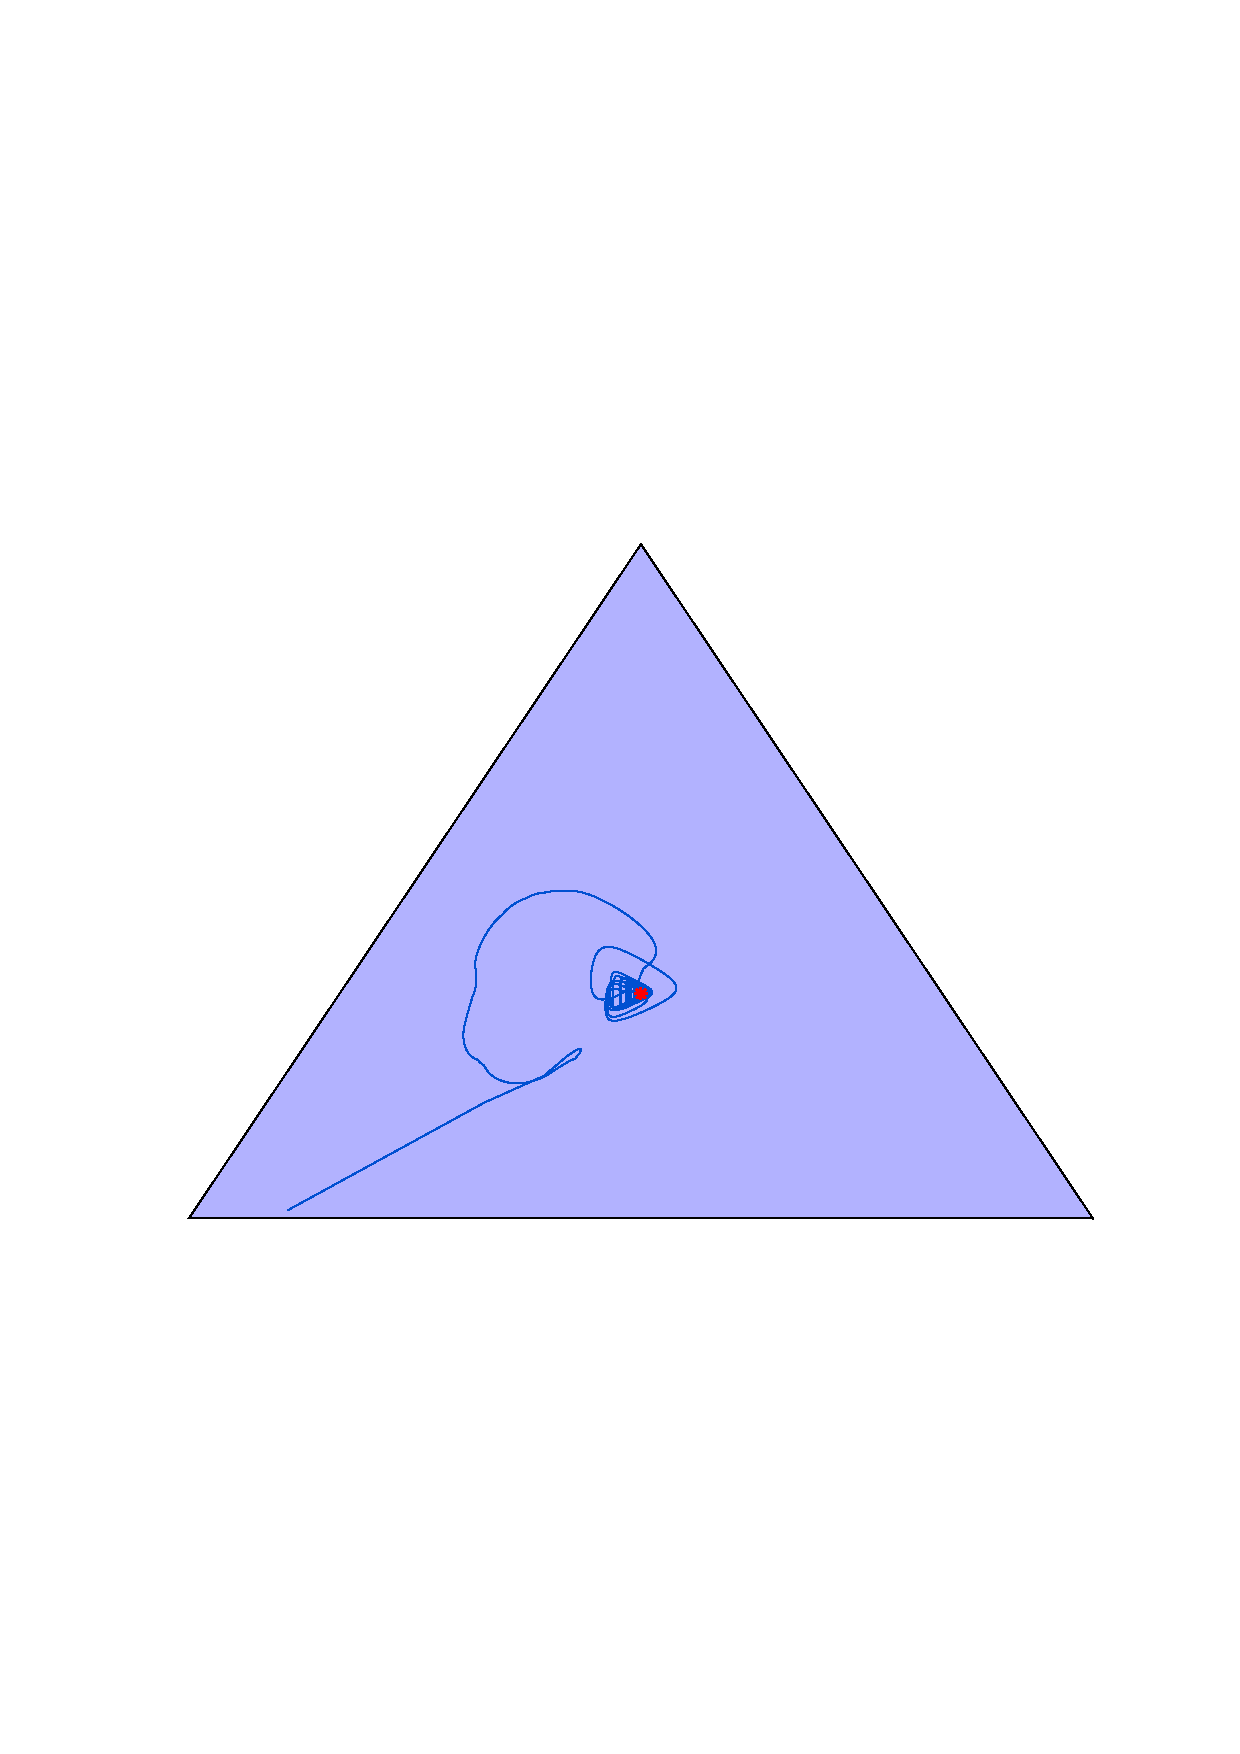
\includegraphics[width=8cm]{./img/rps_ewm.pdf}
\caption{Rock Paper Scissor Dynamics Exponentially Weighted Majority}
\label{fig:RPS}
\end{figure}

\section{Online Convex Optimization for Regret Minimization}\label{sec:OCO}

Let's compare this framework to an apparently unrelated problem, namely optimization, this will be the most suited framework to embed the Online Portfolio Optimization Problem. In online optimization an agent $\mathcal A$ is set to optimize a sequence of functions $f_t(x)$ where usually $f_t:\mathcal X\to \mathbb R$ is a real valued function from the set $\mathcal X\subset\mathbb R^n$. IN Online Convex Optimization literature, some times the loss functions are identified as $f(x,y_t)\equiv f_t(x)$.
The decision space $\mathcal D$ is assumed to be convex, as the are the functions $f_t:\mathcal D\to \mathbb R$. This framework was first devised in \cite{zinkevich2003online}, and has been later wildly used in the machine learning community to engineer optimization procedures \cite{shalev2012online}. 

Convexity plays an central role in most of the analysis made in Online Learning, and Online Convex Optimization. Convexity of the domain $\mathcal D$ and of the loss functions, $f(\cdot,r)$ bound the problem geometry and let us derive simple and efficient learning procedures. More generally in the subsequent section we will present the general learning.

\subsection{A General Algorithm for Online Convex Optimization}

In this Section we will see an algorithm called \emph{Online Mirror Descent} (OMD), that generalizes many Online Convex Optimization algorithms. It is a first order method that works in the dual space defined by the choice of some regularizator \todo{regularizator?}. The OMD algorithm is genral and optimal in the sense that every Online Convex problem can be learned online nearly optimally with OMD, the precise formulation can be found in \cite{srebro2011universality}.

OMD works with a class of regularitators called Bregman Divergences, \cite{banerjee2005clustering}.

\begin{definition}(Bregman divergence). Given a differentiable convex function $\psi:\mathcal X\to\mathbb R$ the Bregman divergence is defined as an operator $d_{\psi}:\mathcal X\times\mathcal X\to \mathbb R^+$ defined for $x,y\in\mathcal X\times\mathcal X$ as 
\begin{equation}\label{eq:bregman_div}
d_\psi(x,y)=\psi(x)-\psi(y)-\langle x-y,\nabla \psi(y)\rangle
\end{equation}
\end{definition}

Since $\psi$ is convex we have that $d_\psi(x,y)\ge0$, we can see that by linearization of $\psi(x)$ around $y\in\mathcal X$ and by the inequality on the non standard inner product defined by the hessian of the function $\psi$ which is positive thanks to the convexity. Since the operator defined in Equation \eqref{eq:bregman_div} is not symmetric in its arguments, it does not define an metric in the space $\mathcal X$.

For $\psi(x)=||x||_2^2$ then $d_\psi(x,y)=||x-y||_2^2$. For $\psi(x)=\sum\limits_{i=1}^Nx_i\log(x_i)$ then $d_\psi(x,y)=\sum\limits_{i=1}^Nx_i\log(x_i/y_i)$, for $x,y\in\Delta_{N-1}\subset \mathbb R^N$ which is the well know Kullback–Leibler divergence~\cite{van2014renyi}.

The OMD algorithm for Online Convex Optimization, uses the regularization given by a Bregman divergence to follow the best point in the convex set $\mathcal D$ up to now, but it is kept close to the current one by the divergence operator. Formally:

\begin{definition}(Online Mirror Descent). OMD for a Bregamn Divergence induced by the differentiable, convex real values function $\psi$, and for a set of learning rates $\{\eta_0,\ldots,\eta_T\}$ has the following update rule: 
$$x_{t+1} =\arg\min\limits_{x\in\mathcal X} d_\psi(x,x_t)+\eta_t\langle\nabla f_t(x_t),x-x_t\rangle,$$
\end{definition}

Next we will show the idea for a general bound for the OMD algorithm, this is to show the geometric ideas behind the OMD algorithm. It is important to point that the analysis can be refined by fixing the loss function $f_t$ or the convex function $\psi$.

The convex function $\psi$ is assumed to be differentiable in the domain $\mathcal X$, but it is not required by the analysis, and in general we can work with subgradients rather than gradients. \todo{chiarire o togliere completamente}  

\begin{theorem}\label{th:OMD_first_th}
Let $d_\psi:\mathcal X\times\mathcal X\to \mathbb R$ the Bregman divergence associated to the convex smooth function $\psi$. Moreover, assume $d_\psi$ is $\alpha$-strong convex, \emph{i.e.} $d_\psi(x,y)\ge\frac{\alpha}{2}||x-y||^2$.
Then $\forall x\in\mathcal X$ we have 
$$\eta_t (f_t(x_t)-f_t(x))\le d_\psi(x,x_t)-d_\psi(x,x_{t+1})+\frac{\eta_t^2}{2}||\nabla f_t(x_t)||_*^2$$ 
\end{theorem}
\todo{proof or not?}

Theorem \ref{th:OMD_first_th} can be used to prove a regret bound for the general OMD algorithm. 

\begin{theorem}(Regret Bound for Online Mirror Descent).
\end{theorem}




% \begin{algorithm}[t!]
%     \caption{OGD in OPO with Transaction Costs}
%     \label{alg:OGD_in_OPO}
%     \begin{algorithmic}[1]
%     \REQUIRE learning rate sequence $\{\eta_1, \ldots, \eta_T\}$  \nonumber
%     \STATE Set $\mathbf{x}_1 \gets \frac{1}{M} \mathbf{1}$ \label{line:init}
%     \FOR {$t \in \{ 1, \ldots, T \}$}
%     \STATE Select portfolio $\mathbf{x}_{t+1} \gets \Pi_{\Delta_{M-1}}\left(\mathbf{x}_{t}+ \eta_t \frac{\mathbf{r}_t}{\langle \mathbf{r}_t,\mathbf{x}_t \rangle}\right)$ \label{line:update}
%     \STATE Observe $\mathbf{r}_{t+1}$ from the market \label{line:out}
%     \STATE Get wealth $\log( \langle \mathbf{r}_{t+1},\mathbf{x}_{t+1} \rangle) - \gamma|| \mathbf{x}_{t+1} - \mathbf{x}_{t} ||_1$ \label{line:wealth}
%     \ENDFOR
%     \end{algorithmic}
% \end{algorithm}

\subsection{Statistical Learning and Online Learning}
\todo{cita}
Now we explore the connection between the Online Optimization framework and classical concepts of classical Statistical Learning techniques. More concretely we can prove and design a whole class of algorithm that are Agnostically PAC Learnable with Online Learning Techniques.
Classical statistical learning theory deals with examples (or observations) and models of the phenomena. Then it uses the model to predict the future observations~\cite{bousquet2003introduction}. Quite informally one could say that we are trying to infer concept from examples. A concept is a map $\mathcal C:\mathcal X\to\mathcal Y$, where $X$ is the domain space and $\mathcal Y$ is the set of labels for the examples. We then observe a sample from an unknown distribution $\mathcal D$ such that $(x,y)\sim \mathcal D$. What we need to achieve is to learn a mapping $y:\mathcal X\to\mathcal Y$ such that the error under the distribution $\mathcal D$ is small. The loss function needed to define this error is not specific to the problem and can be decided by the user, this is called generalization error and, for a loss function $l:\mathcal Y\times\mathcal Y \to\mathbb R$, it is defined as:
\begin{equation}\label{eq:generalization}
    e(h) = \mathbb E_{(x,y)\sim \mathcal D}[l(h(x),y)]
\end{equation}
The goal for an algorithm $\mathcal A$ is to produce a hypothesis $h$ with small generalization error. 
It is generally difficult to generalize well and how difficult is clarified by the following theorem called the \emph{No free lunch theorem} \todo{quale cit?}. There are many variation of this theorem, there is one formulation which states that: for any learner $\mathcal A$ that learns an hypothesis $h:\mathcal X\to \{0,1\}$, there exists a concept $\mathcal C$ with generalization error $0$ and a distribution $\mathcal D$ such that the generalization error of $\mathcal A$ is at least $1/2-\epsilon$ for any $\epsilon>0$. Hence it is impossible to learn any concept in this general sense. But we can learn concept restricting the class of concepts in a hypothesis space $\mathcal H:\mathcal X\to\mathcal Y$.
This restriction gives raise to the concept of Probably Approximately Correct (PAC) learnability. 

\begin{definition}(PAC learnable).\label{def:PAC}
    An hypothesis class $\mathcal H$ is PAC learnable w.r.t. the loss $l$ if there exists a learner $\mathcal A$ that given a sample $S_N$ of examples learns an hypothesis $h\in\mathcal H$ s.t. for all $\epsilon,\delta$ there exists $N_{\epsilon,\delta}$ such that for any distribution $\mathcal D$ we have a generalization error $\mathbb P[e(h)<\epsilon]\ge1-\delta$
\end{definition}

Usually we also require that the algorithm $\mathcal A$ learns the concept $h$ in polynomial time w.r.t. the parameter of the problem. 

An example of such learning problems could be the classification of spam emails. In this case $\mathcal X$ is the vectorial representation of the text and $\mathcal Y=\{0,1\}$, indicating weather or not the email it a spam or not. If we choose as a model a linear classifier then the hypothesis space is $\mathcal H=\{h = \mathbb I[\langle x,w\rangle \ge 1/2]\}$ and the loss could be chose as $l(y_1,y_2)=|y_1-y_2|$.

PAC learnability is intuitively requiring that the there exists an hypothesis $h\in\mathcal H$ with near zero generalization error, otherwise the class $\mathcal H$ is not PAC learnable, otherwise the class $\mathcal H$ is not PAC learnable.
But we can weaken the concept of PAC learnability by addressing directly this issue.

\begin{definition}(PAC agnostic learnable).
    Given the same definitions of Definition \ref{def:PAC}, an hypothesis class $\mathcal H$ is PAC agnostic learnable if we have a generalization error $\mathbb P[e(h)<\inf\limits_{\tilde h\in\mathcal H}e(\tilde h)+\epsilon]\ge1-\delta$
\end{definition}

Which hypothesis spaces $\mathcal H$ are PAC learnable (agnostically or not) is an open and complex issue, but the case for convex hypotheses class $\mathcal H\subset\mathcal R$ can be solved by Online Learning techniques, showing the versatility of the methods. 
Moreover approach to prove such theorem gives an constructive methodology to solve agnostic PAC learnable problems.

\begin{theorem}
For every hypothesis class $\mathcal H$ and bounded loss function $l:\mathcal Y\times\mathcal Y\to \mathbb R$, for which does exists a low regret algorithm $\mathcal A$, then the problem is angostic PAC learnable. In particular this conditions are satisfied if the hypotesis space $\mathcal H$ and the loss function $l$ are convex.
\end{theorem}

\begin{proof}(Sketch).
Initialize the learner with the hypothesis $h_0=\mathcal H$.
For every iteration $t\le T$: observe a sample $(x_t,y_t)\sim\mathcal D$ and a loss function $l_t:=l(h_t(x_t),y_t)$. Then update the hypotesis $h_{t+1}=\mathcal A(l_1,\ldots,l_t)$.

At $t=T$ return $\bar{h}=\frac{1}{T}\sum\limits_{t=1}^T h_t\in\mathcal H$. 

The proof then continues by defining the random variable $X^{(1)}_T=\sum\limits_{t=1}^Te(h_t)-l(h_t(x_t),y_t)$ this is a martingale and $\mathbb E[X^{(1)}_T]=0$. Moreover $|X^{(1)}_T-X^{(1)}_{T-1}|<K$ since the loss function $f$ is bounded. We can normalize the losses so that $K=1$, and then apply the Azuma martingale inequality $\mathbb P[X^{(1)}_T>c]\le e^{-\frac{c^2}{2T}}$.

For an appropriate choice of $c$ we get

\begin{equation}\label{eq:ineq_1_APCA}
\mathbb P\left[\frac{1}{T}\left[\sum\limits_{t=1}^Te(h_t)-l(h_t(x_t),y_t)\right)>\sqrt{\frac{2\log(\delta/2)}{T}}\right]\le \delta/2
\end{equation}
defining $h^*=\arg\inf\limits_{h\in\mathcal H} e(h)$ and $X^{(2)}_T=\sum\limits_{t=1}^Te(h^*)-l(h^*(x_t),y_t)$ we can obtain
\begin{equation}\label{eq:ineq_2_APCA}
\mathbb P\left[\frac{1}{T}\left(\sum\limits_{t=1}^Te(h^*)-l(h^*(x_t),y_t)\right)<-\sqrt{\frac{2\log(\delta/2)}{T}}\right]\le \delta/2
\end{equation}

By the definition of regret $y_T$ we obtain

\begin{equation}\label{eq:eq_regret_APAC}
\frac{1}{T}\sum\limits_{t=1}^Te(h_t)-e(h^*)=y_T/T+X_T^{(1)}-X_T^{(2)}
\end{equation}

and from inequalities \eqref{eq:ineq_1_APCA}, \eqref{eq:ineq_2_APCA} and from Equation \eqref{eq:eq_regret_APAC} we have:

\begin{equation}
\mathbb P\left[\frac{1}{T}\sum\limits_{t=1}^Te(h_t)-e(h^*)>\frac{y_T}{T}+2\sqrt{\frac{2\log(\delta/2)}{T}}\right]\le \delta
\end{equation}

Now simply thanks to the linearity of the error operator $e:\mathcal H\to \mathbb R$ we have that 

$$\mathbb P\left[e(\bar h)<e(h^*)+y_T/T+2\sqrt{\frac{2\log(\delta/2)}{T}}\right]\le 1-\delta$$
and since $y_T/T\to0$ we can find $\tilde T$ large enough such that the thesis is verified.
\end{proof}

This result has been presented since it is useful to prove the general behavior of Hannan consistent strategies in environments driven by a stationary distribution.
\chapter{Information, Prediction and Investing}

In Chapter \ref{ch:OnlineLearning} we described at a high level the framework of Online Learning in Adversarial environment. Now we draw the connections between that and predictions. It surly seems counter intuitive to speak about predictions in an adversarial framework, since we are used to think about predictions only of stochastic processes. The root of this formulation are to be traced back to the Bell Laboratories in the '50, from works of Kelly \cite{kelly2011new}, linking sequential betting and information rate. This connection is of primary importance to understand sequential investing as an instance of sequential decision problem.
We first draw the parallelism between probability assignment over discrete events and Online Learning and then extend the discussion to sequential investments.

\section{Probability assignment}
The decision space $\mathcal D$ in the case of finite $N$ possible bets is the $\Delta_{N-1}\subset \mathbb R^{N}$ probability simplex while the outcome $\mathcal Y$ space is the set $\{1,\ldots,N\}$, representing the winning bet at each turn. The loss function $f(x,y)$ should have these natural properties: low when $x_y~1$ and high when $x_y~0$ where $x_y$ is the probability assigned to the outcome $y$. The inverse log-likelihood seems a reasonable proposal, simply because the multiplicative additive property of the logarithm but has also a deeper connection to information that we will discuss later on:

\begin{definition}(Self Information Loss).
    In the sequential probability assignment problem the loss function $f(x,y)$, $x\in \Delta_{N-1}$ and $y\in[1,\ldots,N]$ is defined as
    $$f(x,y)=-\log(x_y)$$
where $x_y$ is the probability assigned to outcome $y\in\mathcal Y$.
\end{definition}

In the case of simulable experts, the prediction $x_t$ of the agent is a function of the history of outcomes $y^{t-1}:=\{y_1,y_2,\ldots,y_{t-1}\}\in\mathcal Y^{t-1}$. An expert can be thought of as a set of functions $g_k:\mathcal Y^{k-1}\to\Delta_{N-1}$.




\chapter{Algorithms for the Online Portfolio Optimization Problem}

In this section we will review the state of the art algorithms for the Online Portfolio Optimization problem and discuss their theoretical guarantees.


\chapter{Algorithms for the Online Portfolio Optimization Problem}\label{ch:algos}

In this section we will review the state of the art algorithms for the Online Portfolio Optimization problem and discuss their theoretical guarantees, and how these algorithms can be generated by the theoretical framework of Online Learning with expert advice and Online Optimization we described in Chapter \ref{ch:OnlineLearning}.

The setting is the one described in Section \ref{sec:OPO}, in particular $\Delta=\Delta_{N-1}\subset \mathbb R^N$ is the $N$-simplex, and an element $\mathbf x_t\in\Delta$ describes the allocation over $N$ stocks for the $t$-th period.

As is commonly done in the portfolio allocation literature~\cite{agarwal2006algorithms}, we assume that the price of the assets does not change too much during two consecutive rounds, or, formally:

\begin{assumption} \label{ass:nojunk}
    %  Given the OPO framework, 
     There exist two finite constants $\epsilon_l, \epsilon_u \in \mathbb{R}^+$ s.t.~the price relatives~$y_{j,t} \in [\epsilon_l, \epsilon_u]$, with $0 < \epsilon_l \leq \epsilon_u < +\infty$, for each round $t \in \{ 1, \ldots, T \}$ and each asset $j \in \{1, \ldots, N \}$.
\end{assumption}

Notice that under Assumption~\ref{ass:nojunk} it is possible to bound the $L_1$, $L_2$ and the $L_\infty$ gradient of the loss as follows:\todo{check}

\begin{equation} \label{eq:bounded_gradient_1}
    ||\nabla \log (\langle \mathbf{x}_t, \mathbf{y}_t) \rangle||_1 \leq \frac{N\epsilon_u}{\epsilon_l}:=G_1,
\end{equation}

\begin{equation} \label{eq:bounded_gradient_2}
    ||\nabla \log (\langle \mathbf{x}_t, \mathbf{y}_t) \rangle||_2 \leq \frac{\epsilon_u \sqrt{N}}{\epsilon_l}:=G_2,
\end{equation}

\begin{equation} \label{eq:bounded_gradient_3}
    ||\nabla \log (\langle \mathbf{x}_t, \mathbf{y}_t) \rangle||_\infty \leq \frac{\epsilon_u }{\epsilon_l}:=G_\infty.
\end{equation}

Since we will compare multiple algorithms, we introduce the notation $R_T(\mathcal A)$ when speaking about the regret at time $T$ of an online learner $\mathcal A$. The same notation applies with the total regret $R_T^C$ or the regret on the costs $C_T$, defined in Section \ref{ch:transaction_costs}.

\section{Algorithm with regret bound}

As already pointed out, most algorithms in the Online Portfolio Optimization literature do not consider transaction costs and have guarantees only on the standard regret $R_T$. In this section we will summarize the most relevant algorithms for the Online Portfolio Optimization problem that have been proven to have only bounded regret $R_T$. 

\subsection{Universal Portfolios}\label{sec:UP}
The Universal Portfolios (UP) \cite{cover1996universal} algorithm has been one of the first algorithms that have been introduced in the framework of Online Portfolio Optimization. The UP algorithm has the best theoretical guarantees among the algorithm for Online Portfolio Optimization, as it can reach the minmax value of the game between the adversarial environment and the learning agent (Theorem 10.2 \cite{cesa2006prediction}).


\begin{definition}(Universal Portfolios).
The prediction of the UP algorithm is the following:
\begin{equation}\label{eq:UP}
\mathbf x_{t+1}=\frac{\int_{\Delta}\mathbf x W_t(\mathbf x)d\mathbf x}{\int_{\Delta} W_t(\mathbf x)d\mathbf x}.
\end{equation}
\end{definition}

Note that this algorithm is the Continuous Mixture Forecaster for exp-concave losses, described in Section \ref{sec:exp-concave-mixture}, since the logarithmic loss is exp-concave with $\nu=1$. as described in the analysis of Section \ref{sec:laplace_mixture}.

Hence, we have that: 
\begin{equation}
R_T(UP)\le(N-1)\log(T+1).
\end{equation}

Clearly the UP algorithm is computationally hard as it involves integration over a $N$-simplex. Indeed, there is an extensive research that looks into efficient implementations of the UP algorithm \cite{kalai2002efficient}.


Moreover, the update rule in Equation \eqref{eq:UP} can be generalized as follow:

\begin{equation}\label{eq:general_UP}
\mathbf x_{t+1}=\frac{\int_{\Delta}\mathbf x W_t(\mathbf x)\mu(\mathbf x)d\mathbf x}{\int_{\Delta} W_t(\mathbf x)\mu(\mathbf x)d\mathbf x},
\end{equation}

where $\mu(\mathbf x)$ is a distribution over $\Delta_{N-1}$, the standard UP algorithm is obtained by choosing $\mu$ as the uniform distribution over the probability simplex, but there are choices of $\mu(\mathbf x)$ for which we can obtain slightly better constants for the regret bound.

% \subsection{Implementation of Universal Portfolios}

% To implement Universal Portfolio


\subsection{Exponential Gradient}

The Exponential Gradient (EG) algorithm is a specification of the OMD algorithm described in Section \ref{sec:OMD}, by using the Kullback–Leibler divergence $d_\psi(\mathbf x,\mathbf y)=KL(\mathbf x,\mathbf y)=\sum\limits_{i=1}^Nx_i\log(x_i/y_i)$ as the Bregman divergence the, and $\eta_t=\eta$ as the constant sequence of learning rates. The update rule for EG in this case becomes:

\begin{definition}(Exponential Gradient). The EG algorithm is defined by the following update rule:
\begin{equation}\label{eq:update_EG}
\mathbf x_{t+1}=\arginf\limits_{\mathbf x\in\Delta_{N-1}} \left\{KL(\mathbf x,\mathbf x_t)-\eta_t\left\langle \frac{\mathbf x_t}{\langle \mathbf x_t,\mathbf y_t\rangle},\mathbf x-\mathbf x_t\right\rangle\right\}.
\end{equation}
\end{definition}

The update rule in Equation \eqref{eq:update_EG} can be solved analytically \cite{helmbold1998line}, giving the following closed update 

\begin{equation}\label{eq:update_EG_closed}
x_{i,t+1}=\frac{x_{j,t}\exp\left(\eta_t{y_{j,t}}/\langle\mathbf x_t,\mathbf y_t\rangle\right)}{\sum\limits_{j=1}^Nx_{j,t}\exp\left(\eta_t{y_{j,t}}/\langle\mathbf x_t,\mathbf y_t\rangle\right)}, \forall i\in1,\ldots,N.
\end{equation}

This update rule is also a Weighted Average Forecaster described in Section \ref{sec:existence_of_no_regret}, and in particular, it is a special case of Exponentially Weighted Forecaster of Definition \ref{def:ewf}. This is useful for proving the following theorem.

\begin{theorem}(Regret Bound for the Exponential Gradient Algorithm).
The EG algorithm defined by the update rule in Equation \eqref{eq:update_EG_closed} has the following regret bound:
\begin{equation}
R_T(EG)\le \frac{\epsilon_u}{\epsilon_l}\sqrt{\frac{T\log N}{2}}.
\end{equation}
\end{theorem}

\begin{proof}
We know that $\psi(\mathbf x)=\sum\limits_{i=1}^Nx_i\log(x_i)$ is $1$-strong convex with respect to the $L_1$ norm $||\cdot||_1$ \cite{shalev2007online}, and so we have that $KL(\mathbf x,\mathbf x_t)\ge\frac{1}{2}||\mathbf x-\mathbf x_t||_1$.

Moreover, we can bound the $L_1$ diameter $D_1$ of the simplex $\Delta_{N-1}$ as: 
$$D_1=\sup\limits_{\mathbf x,\mathbf y\in\Delta_{N-1}}||\mathbf x-\mathbf y||_1\le2.$$

Therefore, we can apply Theorem \ref{th:regret_omd} with $\eta=\frac{1}{G_\infty}\sqrt{\frac{2\log N}{T}}$ and $\mathbf x_1=(1/N,\ldots,1/N)$ giving as a result the thesis.
\end{proof}

Note that one could also obtain a regret bound by using the fact that the EG algorithm is a specialization of OMD with $\psi(\mathbf x)=\sum\limits_{i=1}^N x_i\log(x_i)$ 


\subsection{Online Newton Step}

The Online Newton Step (ONS) \cite{hazan2007logarithmic} algorithm is one of the few algorithms other than the UP one, that guarantees a logarithmic bound $R_T(ONS)=\mathcal O(\log T)$. The method uses second order information of the loss function, but it can nonetheless be stated into first order method such as OMD, as we will discuss at the end of this section.

\begin{definition}(Online Newton Step).
The ONS algorithm is defined by the following update rule:
\begin{equation}\label{eq:update_ONS}
\mathbf x_{t+1}=\Pi^{A_t}_{\Delta_{N-1}}\left(\mathbf x_t+\frac{1}{\beta}A_t^{-1}\frac{\mathbf y_t}{\langle\mathbf x_t,\mathbf y_t\rangle}\right),
\end{equation}
where $\prod^{A_t}_{\Delta_{N-1}}(\cdot)$ is the non-standard projection onto the simplex $\Delta_{N-1}$ defined as 
\begin{equation}\label{eq:non_standard_proj}
\Pi^{A_t}_{\Delta_{N-1}}(\mathbf x_0):=\arginf\limits_{\mathbf x\in\Delta_{N-1}}\langle\mathbf x-\mathbf x_0,A_t(\mathbf x-\mathbf x_0)\rangle,
\end{equation}

and the matrix $A_t\in\mathbb R^{N\times N}$ is defined as 
\begin{equation}\label{eq:matrix_ONS}
A_t=\sum\limits_{s=1}^t \nabla f_t(\mathbf x_t)\nabla f_t(\mathbf x_t)^T+\epsilon\mathbb I_N,
\end{equation},
where $\mathbb I_N$ si the identity matrix in $\mathbb R^N$.
\end{definition}

The idea for the ONS algorithm is originated from the concept of strong convexity, that is defined as follow:

\begin{definition}(Strong Convexity).\label{def:strong_cnvx}
A function $f:\mathcal D\to\mathbb R$ is said to be $\mu$-strong convex w.r.t. the norm $||\cdot||$ if: 
$$f(y)-f(x)\ge\langle\nabla f(x),y-x\rangle+\frac{\mu}{2}||y-x||^2,\forall x,y\in\mathcal D,\forall x,y\in\mathcal D.$$
\end{definition}

Usually there is the correspondence of convex-loss $R_T=\mathcal O(\sqrt T)$ and strong-convex loss $R_T=\mathcal O(\log T)$. The idea of the ONS algorithm is to recover a weaker concept of strong convexity for exp-concave losses:

\begin{definition}(Weak Strong Convexity).\label{def:weak_strong_cnvx}
A function $f:\mathcal D\subset \mathbb R^N\to\mathbb R$ is said to be weak-strong convex if $\forall x\in\mathcal D\exists A\in\mathbb R^{N\times N}$ such that: 
$$f(y)-f(x)\ge\langle\nabla f(x),y-x\rangle+\frac{\mu}{2}||y-x||_{A}^2,$$
for a positive defined matrix $A$ that defines the norm $||x||^2_{A}=\langle x, Ax\rangle$.
\end{definition}

Indeed, for any $\nu$ exp-concave function $f:\mathcal D\to\mathbb R$ with bounded gradient, \emph{i.e.} $||\nabla f(\mathbf x)||_2\le G\ \forall \mathbf x\in\mathcal D$, with $D=\sup\limits_{\mathbf x,\mathbf y\in\mathcal X}||\mathbf x-\mathbf y||_2$, $\beta=\frac{1}{2}\min\{\nu,\frac{1}{4GD}\}$ and $A=\nabla f(\mathbf x)\nabla f(\mathbf x)^T$, we have that: 

\begin{equation}\label{eq:weak_strong_conv_exp_concave}
f(\mathbf y)-f(\mathbf x)\ge\langle\nabla f(x),\mathbf y-\mathbf x\rangle+\frac{\beta}{2}||\mathbf y-\mathbf x||_{A}\forall x,y\in\mathcal D.
\end{equation}

The main idea of ONS is exploiting the weak-strong convexity of exp-concave functions to recover $\mathcal O(\log T)$ regret bounds. The complete proof can be found in \cite{hazan2007logarithmic}.

From Equation \eqref{eq:weak_strong_conv_exp_concave} we can see that the matrix $A$ used by the ONS algorithm is just a lower bound on the Hessian of the loss function. This is also the reason why the projection onto the simplex of the ONS algorithm is the non standard projection defined by the matrix $A_t$ defined in Equation \eqref{eq:matrix_ONS}.

\begin{theorem}(Regret Bound for the Online Newtonw Step Algorithm).

By choosing $\beta=\frac{\alpha}{8\sqrt{N}}$ in Equation \eqref{eq:update_ONS}, the regret bound for the ONS algorithm becomes:

\begin{equation}\label{eq:regret_ONS}
R_T(ONS)\le\frac{10 N^{3/2}}{\epsilon_l}\log\left(\frac{NT}{\epsilon_l^2}\right)
\end{equation}
\end{theorem}

ONS can also be seen as a specification of OMD \cite{luo2018efficient} by choosing an adaptive regularizer $\psi(\mathbf x)=\psi_t(\mathbf x)=\frac{1}{2}||\mathbf x||_{A_t}^2$ where $A_t$ is defined as $A_t=A_{t-1}+\nabla f_t(\mathbf x_t)\nabla f_t(\mathbf x_t)^T$, for a positive defined $A_0$. In this case the gradient of the Fenchel Conjugate becomes $\nabla \psi_t^*(\mathbf x)=\Pi^{A_t}_{\Delta_{N-1}}(\mathbf x)$, defined in Equation \eqref{eq:non_standard_proj}.

\section{Algorithm with total regret bound}

To the best of our knowledge there are only two works that bound the total regret $R_T^C$ defined in Chapter \ref{ch:transaction_costs}. We will present the works and discuss their limitations, that we tried to solve with our approach.

\subsection{Online Lazy Updates}

Online Lazy Updates (OLU) \cite{das2013online} is an algorithm designed to minimize explicitly the total regret $R_T^C$. The origin of this algorithm has to be traced back to a generalization of the OMD algorithm discussed in Section \ref{sec:OMD}. Namely, the generalization of the OMD algorithm that we are referring to is the Composite Objective Mirror Descent (COMID) algorithm \cite{duchi2010composite}. The idea behind the COMID algorithm is to have a composite loss function of the kind $g_t(\mathbf x)=f_t(\mathbf x) + r(\mathbf x)$, then the algorithm linearizes the first term $f_t(\mathbf x)$ of the composite loss (as in OMD) but does not linearize the second term $r(\mathbf x)$ of the composite loss $g_t(\mathbf x)$. Both terms of the loss function, $f_t$ and $r$, are assumed to be convex.

\begin{definition}(Composite Objective Mirror Descent).\label{def:COMID}
The COMID algorithm is defined with the following update equation:
\begin{equation}\label{eq:update_COMID}
    \mathbf{x}_{t+1}=\arginf\limits_{\mathbf{x} \in \Delta_{M-1}} \hspace{-0.1cm} \left\{ \eta \langle \nabla f_t(\mathbf{x}_t), \mathbf{x} \rangle + \eta \ r(\mathbf{x}) + d_\psi(\mathbf{x}, \mathbf{x}_t) \right\},
\end{equation}

where $d_\psi$ is the Bregman divergence for a convex function $\psi$. 

\end{definition}

A lemma similar to Lemma \ref{th:OMD_first_th} gives the following guarantees to the regret of a learner using COMID:

\begin{lemma}(\cite{duchi2010composite} Theorem 2.2)
$\forall \mathbf x\in\Delta_{N-1}$ and for a sequence $\{\mathbf x_t\}_{t=1}^T$ defined by the update rule \eqref{eq:update_COMID}, we have:
\begin{equation}
\eta\sum\limits_{t=1}^T[f_t(\mathbf x_t)-f_t(\mathbf x)+r(\mathbf x_t)-r(\mathbf x)]\le d_\psi(\mathbf x,\mathbf x_t)+\eta r(\mathbf x_1)+\frac{\eta^2}{2\alpha}\sum\limits_{t=1}^T||\nabla f_t(\mathbf x_t)||_*^2,
\end{equation} 
where $\alpha$ is the parameter that ensures $d_\psi(\mathbf x,\mathbf y)\ge \frac{\alpha}{2}||\mathbf x-\mathbf y||^2$.
\end{lemma}

This lemma implies a regret bound on $R_T$. If we assume that the losses $f_t$ have bounded gradient by $G_*$ under the norm $||\cdot||_*$ then we have that: 

\begin{equation}
\sum\limits_{t=1}^T[f_t(\mathbf x_t)-f_t(\mathbf x)+r(\mathbf x_t)-r(\mathbf x)]\le\frac{1}{\eta}d_\psi(\mathbf x,\mathbf x_t)+r(\mathbf x_1)+\frac{T\eta}{2\alpha}G_*^2.
\end{equation}

Consequently, taking $\eta=\frac{K}{\sqrt T}$, and assuming $d_\psi(\mathbf x,\mathbf y)\le D\ \forall\mathbf x,\mathbf y\in\Delta_{N-1}$, and $r(\mathbf x_1)\le D_1$, we obtain:

\begin{equation}\label{eq:regret_comid_final}
\sum\limits_{t=1}^T[f_t(\mathbf x_t)-f_t(\mathbf x)+r(\mathbf x_t)-r(\mathbf x)]\le KD\sqrt{T} + D_1+\frac{\sqrt{T}}{2\alpha}G_*^2.
\end{equation}

The idea of OLU is to take $r=r_t(\mathbf x)=\gamma||\mathbf x-\mathbf x_{t-1}||_1$ \cite{das2014online}, $\psi=||\mathbf x||_2^2$ generating the following update rule:

\begin{definition}(Online Lazy Update).\label{def:update_OLU}
The OLU algorithm is defined by the following update rule:
\begin{equation}\label{eq:update_OLU}
    \mathbf{x}_{t+1}=\arginf\limits_{\mathbf{x} \in \Delta_{M-1}} \hspace{-0.1cm} \left\{ -\eta\log(\langle \mathbf x,\mathbf y_t\rangle) + \eta \gamma ||\mathbf x_t-\mathbf x||_1 + \frac{1}{2}||\mathbf x-\mathbf x_t||^2_2 \right\}.
\end{equation}

\end{definition}

Note that there are multiple definitions of the OLU algorithm, and we reported a version in which the first term of the loss has not been linearized. Linearization of the first term of the loss with $\langle\nabla f_t(\mathbf x_t),\mathbf x\rangle$ would result in the same update rule and same analysis (since the loss $f_t$ is convex).

With this specifications we obtain the result from Equation \eqref{eq:regret_comid_final}:

\begin{equation}
\sum\limits_{t=1}^T[f_t(\mathbf x_t)-f_t(\mathbf x)+\gamma||\mathbf x_t-\mathbf x_{t-1}||_1-\gamma||\mathbf x-\mathbf x_{t-1}||_1]\le \left( \frac{1}{K} + \frac{N K \epsilon_u^2 }{2 \epsilon_l^2} \right) \sqrt{T}.
\end{equation}

Then, taking to the left hand side the terms $\gamma||\mathbf x-\mathbf x_{t-1}||_1$, and specializing $f_t(\mathbf x)$ as the log-loss defined for the Online Portfolio Optimization framework, we obtain:

\begin{equation}
\sum\limits_{t=1}^T[f_t(\mathbf x_t)-f_t(\mathbf x)+\gamma||\mathbf x_t-\mathbf x_{t-1}||_1]\le \sum\limits_{t=1}^T\gamma||\mathbf x-\mathbf x_{t-1}||_1+\left( \frac{1}{K} + \frac{N K \epsilon_u^2 }{2 \epsilon_l^2} \right) \sqrt{T}.
\end{equation}

Now the left hand side is equivalent to our Definition \ref{def:totoal_regret} of total regret $R_T^C$. Note that we do not have a sub-linear bound for the total regret yet. In order to recover the sub-linear bound on the total regret $R_T^C$ in \cite{das2014online} (Theorem 1) the authors assume $\gamma=\frac{\gamma_0}{\sqrt{T}}$. With this assumption we can recover the following bound on the total regret for the OLU algorithm:

\begin{equation}
R_T^C(OLU)\le2\gamma_0\sqrt{T}+\left( \frac{1}{K} + \frac{N K \epsilon_u^2 }{2 \epsilon_l^2} \right) \sqrt{T}.
\end{equation}

It is clear from our discussion on the model for Online Portfolio Optimization with transaction costs described in Chapter \ref{ch:transaction_costs} that $\gamma>0$ is fixed and independent on the time horizon $T$ of the investment process. \todo{F: Scriviamola prima questa cosa di $\gamma$ costante}
\todo{add ADMM}

\subsection{Implementation of Online Lazy Update}

Due to the non-smooth $L_1$ term in Equation \eqref{eq:update_OLU}, we need a special optimization procedure. The authors proposed the Alternating Direction Method of Multipliers (ADMM) scheme \cite{boyd2011distributed}, by decoupling the non-smooth term $||\mathbf x_t-\mathbf x||_1$ from the rest of the objective function.
Indeed, Equation \eqref{eq:update_OLU} is equivalent to 
\begin{equation}
\mathbf x_{t+1}=\argmin\limits_{\mathbf x\in\Delta,\mathbf x-\mathbf x_t=\mathbf z}\left\{-\eta\log(\langle\mathbf x,\mathbf y_t\rangle)+\eta\gamma||\mathbf z||_1+\frac{1}{2}||\mathbf x-\mathbf x_t||_2^2\right\}
\end{equation}

The ADMM method is concerned with optimization problems of the kind

\begin{equation}\label{eq:general_ADMM}
\begin{cases}
\inf f(\mathbf x)+g(\mathbf z) \\
s.t.\ A\mathbf x+B\mathbf z=\mathbf c,
\end{cases}
\end{equation}
where $\mathbf x,\mathbf z,\mathbf c\in\mathbb R^N$ and $A,B\in\mathbb R^N$.

Problem \eqref{eq:general_ADMM} has augmented Lagrangian:

\begin{equation}\label{eq:lagrangian_1}
\mathcal L_\rho(\mathbf x,\mathbf z,\mathbf y )=f(\mathbf x)+g(\mathbf x) + \langle\mathbf y,A\mathbf x+B\mathbf z-\mathbf c\rangle +\frac{\rho^2}{2}||A\mathbf x+B\mathbf z-\mathbf c||_2^2.
\end{equation}

Now ADMM solves the Lagrangian problem by iterating over minimization on the primal variables and then doing a dual update (this justifies the name \emph{alternating direction} in ADMM) with the following update rules:

\begin{equation}\label{eq:update_ADMM_1}
\begin{cases}
(\mathbf x^{k+1},\mathbf z^{k+1})=\arginf\limits_{\mathbf x,\mathbf z }\mathcal L_\rho(\mathbf x,\mathbf z,\mathbf y^{(k)})\\
\mathbf y^{(k+1)}=\mathbf y^{(k)}+\rho(A\mathbf x^{k+1}+B\mathbf z^{(k+1)}-\mathbf c)
\end{cases}
\end{equation}

If we define the residual $\mathbf r=A\mathbf x+B\mathbf z-\mathbf c$ and $\mathbf u=\frac{1}{\rho}\mathbf y$ as the scaled dual variable, then the Lagrangian in Equation \eqref{eq:lagrangian_1} turns into 

\begin{equation}\label{eq:lagrangian_2}
\mathcal L_\rho(\mathbf x,\mathbf z,\mathbf u )=f(\mathbf x)+g(\mathbf x) + \frac{\rho}{2}||\mathbf r+\mathbf u||_2^2-\frac{\rho}{2}||\mathbf u||_2^2
\end{equation}
So we can rewrite the update Equations \eqref{eq:update_ADMM_1} as reported in Algorithm \ref{alg:ADMM}.

\begin{algorithm}[!h]
    \caption{Alternating Direction Method of Multipliers}
    \label{alg:ADMM}
    \begin{algorithmic}[1]
    \REQUIRE $f,g,A,B,\mathbf c,\mathbf x^0,\mathbf z^0,\mathbf u^0,\rho$ \nonumber
    \WHILE{Stopping condition not met:}
    \STATE Update the primal variables: 
    $$(\mathbf x^{k+1},\mathbf z^{k+1})=\arginf\limits_{\mathbf x,\mathbf z }\left\{f(\mathbf x)+g(\mathbf z)+\frac{\rho}{2}||A\mathbf x^{(k)}+B\mathbf z^{(k)}-\mathbf c+\mathbf u^{(k)}||\right\}$$
    \STATE Update the dual variable: 
    $$\mathbf u^{(k+1)}=\mathbf u^{(k)}+A\mathbf x^{k+1}+B\mathbf z^{(k+1)}-\mathbf c$$
    \ENDWHILE
    \RETURN $\mathbf x^k,\mathbf z^k$. 
    \end{algorithmic}
\end{algorithm}

Algorithm \ref{alg:ADMM} is know to converge (see \cite{boyd2011distributed} Appendix A).

In order to use ADMM to solve the optimization of OLU in Equation \eqref{eq:update_OLU}, we have do the following identifications at each time $t$:

\begin{equation}
\begin{cases}
f(\mathbf x)&=-\eta\nabla f_t(\mathbf x_t)\\
g(\mathbf z)&=\gamma\eta||\mathbf z||_1 \\
\mathbf z&=\mathbf x-\mathbf x_t\\
A&=\mathbb I_N\\
B&=-\mathbb I_N\\
\mathbf c&=\mathbf x_t
\end{cases},
\end{equation}
and then use Algorithm \ref{alg:ADMM} to solve Equation \eqref{eq:update_OLU}.



% \subsection{Universal Portfolios with Transaction Costs}

% In \cite{blum1999universal} the authors extended the ideas of the UP algorithm \ref{sec:UP} to include transaction costs. The approach is heavily inspired by the results in Online Learning of Section \ref{sec:laplace_mixture}, namely, the Laplace Mixture Forecaster for the log-loss, and it differs substantially with our approach that is inspired by the Online Convex Optimization framework.

% Indeed the Laplace mixture forecaster has the property \cite{cover1996universal} that the wealth of the Laplace Mixture Forecaster is the average wealth of the wealth of the expert class. The idea followed by the authors is to show that is the portfolios in the expert class are paying transaction costs then the regret experienced by the algorithm \todo{vorrei non mettere UCP perché non lo capisco}

\section{Other Related Works}

There are also heuristic algorithms designed to exploit some known phenomena in markets. Among these heuristic algorithm we can find Anticor~\cite{borodin2004can}, PAMR~\cite{li2012pamr}, OLMAR~\cite{li2015moving}, and MRTC~\cite{yang2018reversion}, which in some cases outperform the algorithms described above in terms of empirical performance. 
Remarkably, none of the above algorithms provide guarantees on the regret, and so we will avoid an in-depth description of their mechanism, since we are currently concerned with algorithms that provide theoretical guarantees without assumptions on the distribution of the marker vectors.
\chapter{Online Gradient Descent for Online Portfolio Optimization with Transaction Costs}\label{ch:OGD}

The Online Gradient Descent (OGD) algorithm is one of the first algorithms developed in the field of Online Convex Optimization \cite{zinkevich2003online}. We extended its use to the Online Portfolio Optimization framework and proved that the OGD algorithm has many interesting properties, among which a bound on the total regret $R_T^C$.

\begin{algorithm}
    \caption{OGD in Online Portfolio Optimization with Transaction Costs}
    \label{alg:OGD_in_OPO}
    \begin{algorithmic}[1]
    \REQUIRE learning rate sequence $\{\eta_1, \ldots, \eta_T\}$  \nonumber
    \STATE Set $\mathbf{x}_1 \gets \frac{1}{N} \mathbf{1}$ \label{line:init_OGD}
    \FOR {$t \in \{ 1, \ldots, T \}$}
    \STATE $\mathbf{z}_{t+1} \gets \mathbf{x}_{t}+ \eta_t \frac{\mathbf{y}_t}{\langle \mathbf{y}_t,\mathbf{x}_t \rangle}$ \label{line:update_OGD}
    \STATE Select Portfolio $\mathbf x_{t+1}=\Pi_{\Delta_{N-1}}(\mathbf z_t)$ \label{line:line_projection_OGD}
    \STATE Observe $\mathbf{y}_{t+1}$ from the market \label{line:out_OGD}
    \STATE Get wealth $\log( \langle \mathbf{y}_{t+1},\mathbf{x}_{t+1} \rangle) - \gamma|| \mathbf{x}_{t+1} - \mathbf{x}_{t} ||_1$ \label{line:wealth}
    \ENDFOR
    \end{algorithmic}
\end{algorithm}

\section{Using OGD for Portfolio Optimization} \label{sec:analysis}

This section describes the adaptation of the OGD algorithm to the Online Portfolio Optimization framework and provides a theoretical analysis of such an algorithm in the presence of transaction costs.

\subsection{The OGD Algorithm}
\label{sec:OGD}
The definition of the OGD update rule for a generic convex loss function $f_t(\mathbf{x}_t)$ over a generic convex set $\mathcal D$ is the following:
\begin{equation}\label{eq:OGD_general}
  \mathbf{x}_{t+1} = \Pi_{\mathcal D} \left( \mathbf{x}_t - \eta_t \nabla f_t(\mathbf{x}_t) \right),
\end{equation}
where $\Pi_{\mathcal D} (y) := \arginf\limits_{x \in \mathcal D } || y - x ||_2^2$ is the standard projection of the vector $y$ onto $\mathcal D$, $\eta_t > 0$ is the learning rate at round $t$.
Recalling that in the Online Portfolio Optimization framework the function to be minimized is the loss $f_t(\mathbf{x}_t) = -\log (\langle \mathbf{x}_t, \mathbf{y}_t \rangle )$, the portfolio update rule becomes:
\begin{equation} \label{eq:OGD_port}
   \mathbf{x}_{t+1}= \Pi_{\Delta_{N-1}}\left( \mathbf{x}_t+\eta_t \frac{\mathbf{y}_t}{\langle \mathbf{x}_t, \mathbf{y}_t \rangle}\right).
\end{equation}
The pseudo-code corresponding to the OGD algorithm is presented in Algorithm~\ref{alg:OGD_in_OPO}. 
The algorithm starts with a portfolio $\mathbf{x}_1$ equally allocated among the $N$ available assets (Line~\ref{line:init_OGD}).
Then, for each round $t \in \{ 1, \ldots, T \}$ it rebalances the assets according to Equation~\eqref{eq:OGD_port}, observes the market outcomes $\mathbf{y}_{t+1}$ (Line~\ref{line:out}), and gains a per-round wealth, including costs, of $\log(\langle \mathbf{y}_{t+1},\mathbf{x}_{t+1} \rangle) - \gamma|| \mathbf{x}_{t+1} - \mathbf{x}_{t} ||_1$ (Line~\ref{line:wealth}). The projection in Line \ref{line:line_projection_OGD}, can be implemented very efficiently as we will discuss in Section \ref{sec:implementation} with Algorithm \ref{alg:projection}.

\begin{figure}[ht!]
\centering
\begin{pspicture}(0,-2.35)(6.9,2.35)
\psellipse[linecolor=black, linewidth=0.04, dimen=outer](3.45,-0.4)(3.45,1.95)
\rput[bl](0.4,-0.55){$\mathcal D$}
\psdots[linecolor=black, dotsize=0.14078125](4.9,1.35)
\psline[linecolor=black, linewidth=0.04, arrowsize=0.05291667cm 2.0,arrowlength=1.4,arrowinset=0.0]{->}(4.9,1.35)(3.3,0.55)
\rput[bl](2.3,0.85){$\eta\nabla f_t(\mathbf x_t)$}
\rput[bl](4.7,1.45){$\mathbf x_t$}
\psline[linecolor=black, linewidth=0.04, arrowsize=0.05291667cm 2.0,arrowlength=1.4,arrowinset=0.0]{->}(4.9,1.35)(6.411111,2.15)
\rput[bl](6.6,2.15){$\mathbf z_t$}
\psdots[linecolor=black, dotsize=0.15374984](6.4,2.15)
\psline[linecolor=black, linewidth=0.04, arrowsize=0.05291667cm 2.0,arrowlength=1.4,arrowinset=0.0]{->}(6.3636365,2.0954545)(5.7272725,1.0045455)
\rput[bl](5.2363634,0.6227273){$\mathbf x_{t+1}$}
\end{pspicture}
\caption{Online Gradient Descent.}
\label{fig:OGD}
\end{figure}

Note that OGD is an instance of the OMD algorithm described in Section \ref{sec:OMD}, with $\psi(\mathbf x)=||\mathbf x||_2^2$. Indeed the general update Equation \eqref{eq:OGD_general} is equivalent to:

\begin{align}
	\mathbf x_{t+1}&=\arginf\limits_{\mathbf x\in\Delta}||\mathbf x-\mathbf x_t+\eta_t\nabla f_t(\mathbf x_t)||_2^2\\
	&=\arginf\limits_{\mathbf x\in\Delta}\left(||\mathbf x-\mathbf x_t||_2^2+\eta_t^2||\nabla f_t(\mathbf x_t)||_2^2+2\langle\nabla f_t(\mathbf x_t),\mathbf x-\mathbf x_t\rangle\right).
\end{align}

\begin{figure}[ht!]
\centering
\begin{pspicture}(0,-2.6668491)(5.5673485,2.6668491)
\psbezier[linecolor=black, linewidth=0.04](0.4,-1.223151)(0.7222638,-0.27650103)(3.9077222,2.3008838)(4.9,2.176849060058594)(5.8922777,2.0528142)(5.522264,-0.876501)(5.2,-1.823151)(4.877736,-2.769801)(4.292278,-2.6471856)(3.3,-2.523151)(2.307722,-2.3991163)(0.0777362,-2.1698008)(0.4,-1.223151)
\psdots[linecolor=black, dotsize=0.16](4.9,-0.82315093)
\psdots[linecolor=black, dotsize=0.16](4.1,1.9768491)
\psdots[linecolor=black, dotsize=0.16](0.4,1.376849)
\rput[bl](0.0,0.9768491){$\mathbf x$}
\rput[bl](3.6,2.276849){$\Pi_{\mathcal D}^A(\mathbf x)$}
\rput[bl](4.6,-1.223151){$\mathbf x_0$}
\psline[linecolor=black, linewidth=0.016](0.4,1.376849)(4.1,1.9768491)
\psline[linecolor=black, linewidth=0.016](4.1,1.9768491)(4.9,-0.82315093)
\psline[linecolor=black, linewidth=0.016](0.4,1.376849)(4.9,-0.82315093)
\rput[bl](2.2,-1.723151){$\mathcal D$}
\end{pspicture}
\caption{Generalized Pythagorean Theorem.}
\label{fig:pitagora}
\end{figure}

\vspace{1cm}

Moreover the following lemma is paramount to prove the regret bound for OGD. This lemma establishes the non expansiveness of the projection operator $\Pi_\Delta$:

\begin{lemma}(Generalized Pythagorean Theorem.)\label{lemma:non_expansive}
Let $\mathcal D\in\mathbb R^N$ a convex set, and $A\in\mathbb R^{N\times N}$ a semi-positive defined matrix. Then, for any point $\mathbf x\in\mathbb R^N$, we have:

\begin{equation}
\langle\mathbf x-\mathbf x_0,A(\mathbf x-\mathbf x_0) \rangle\ge\langle\mathbf z-\mathbf x_0,A(\mathbf z-\mathbf x_0)\rangle, \forall\mathbf x_0\in\mathcal D,
\end{equation}
where $\mathbf z=\Pi_{\mathcal D}^A(\mathbf x)=\arginf\limits_{\mathbf y\in\mathcal D}\langle\mathbf y-\mathbf x,A(\mathbf y-\mathbf x)\rangle$.
\end{lemma}

In the case of $A=\mathbb I_{N\times N}$, being $\mathbb I_{N\times N}$ the identity matrix in $\mathbb R^{N\times N}$, we have that $||\Pi_\mathcal D(\mathbf x)-\mathbf x_0||_2^2\le||\mathbf x-\mathbf x_0||_2^2$. Hence, the operator $\Pi_\Delta:\mathbb R^N\to\mathcal D$ is non-expansive. In Figure \ref{fig:pitagora} is represented Lemma \ref{lemma:non_expansive}.

\section{Regret Analysis}

In this section we will analyze both the regret and the total regret of the OGD algorithm in Online Portfolio Optimization. Indeed, we are able to recover sub-linear regret in both cases, without any assumption on the transaction rate parameter.

\subsection{OGD Regret on the Wealth}
We recall that, for a generic convex function $f_t(x)$, it has been shown in~\cite{belmega2018online} that $
R_T(OGD) = \mathcal{O}(\sqrt{T})$ if the loss function $f_t(x)$ is convex, as in our case.
We follow the proof in~\cite{zinkevich2003online} to derive the specific result for the regret of OGD in the Online Portfolio Optimization framework:
\begin{theorem}\label{th:convex_regret_OGD}
    If Assumption~\ref{ass:nojunk} holds, the OGD algorithm with $\eta_t = \frac{K}{\sqrt{t}}$, $\forall K \in \mathbb{R}^+$ has a regret on the wealth of:
    \begin{equation*}
        R_T(OGD) \leq \left( \frac{1}{K} + \frac{N K \epsilon_u^2}{\epsilon_l^2} \right) \sqrt{T}.
    \end{equation*}
\end{theorem}
\begin{proof}
Notice that the $L_2$ diameter of a simplex $\Delta_{N-1}$ is $D = \sqrt{2}$ for any $N$ and that, under Assumption~\ref{ass:nojunk}, it is possible to bound the gradient of the loss as follows:
\begin{equation} \label{eq:bounded_gradient}
    ||\nabla \log (\langle \mathbf{x}_t, \mathbf{y}_t \rangle)||_2 \leq \frac{\epsilon_u \sqrt{N}}{\epsilon_l}:=G_2.
\end{equation}
Given the update in Equation~\eqref{eq:OGD_port} for the OGD algorithm, we have:
\begin{align}
     ||\mathbf{x}_{t+1} - \mathbf{x}^*||_2^2 &= ||\Pi_{\Delta_{N-1}}(\mathbf{x}_t + \eta_t \nabla \log(\langle \mathbf{x}_t, \mathbf{y}_t \rangle)) - \mathbf{x}^*||_2^2 \nonumber\\
    \leq & ||\mathbf{x}^* - \mathbf{x}_t||_2^2-2\eta_t\langle \mathbf{x}_t-\mathbf{x}^*,\nabla \log( \langle \mathbf{x}_t, \mathbf{y}_t \rangle) \rangle \nonumber \\ 
    & + \eta_t^2||\nabla \log( \langle \mathbf{x}_t, \mathbf{y}_t \rangle)||_2^2, \label{eq:magic}
\end{align}
where we used the fact that the projection operator $\Pi_{\Delta_{N-1}}(\cdot)$ is non-expansive (Lemma \ref{lemma:non_expansive}).
Rearranging the terms, we have:
\begin{align*}
    \langle \mathbf{x}^*-\mathbf{x}_t, \nabla \log (\langle \mathbf{x}_t, \mathbf{y}_t \rangle)\rangle\le \frac{1}{2\eta_t}\left( ||\mathbf{x}_t-\mathbf{x}^*||_2^2-||\mathbf{x}_{t+1}-\mathbf{x}^*||_2^2\right) + \frac{\eta_t}{2}G_2^2.
\end{align*}

Using the above inequality and the convexity of the logarithm, we bound the regret $R_T(OGD)$ as follows:
\begin{align*}
     R_T (ODG) &= \sum\limits_{t=1}^T\log (\langle \mathbf{x}^*, \mathbf{y}_t \rangle)-\log (\langle \mathbf{x}_t, \mathbf{y}_t \rangle) \\
    & \le\sum\limits_{t=1}^T\langle\mathbf{x}^*-\mathbf{x}_t,\nabla \log (\langle \mathbf{x}_t, \mathbf{y}_t \rangle)\rangle\\
    &\le\sum\limits_{t=1}^T\left[\frac{1}{2\eta_t}\left(||\mathbf{x}_t-\mathbf{x}^*||_2^2-||\mathbf{x}_{t+1}-\mathbf{x}^*||_2^2\right)+\frac{\eta_t}{2}G_2^2\right]\\
    &\le\frac{1}{2\eta_1}||\mathbf x^*-\mathbf x_1||_2^2-\frac{1}{2\eta_T}||\mathbf x^*-\mathbf x_{T+1}||_2^2+\sum\limits_{t=2}^T\frac{1}{2\eta_t}||\mathbf x_{t}-\mathbf x^*||_2^2\\
    &-\sum\limits_{t=1}^{T-1}\frac{1}{2\eta_t}||\mathbf x_{t+1}-\mathbf x^*||_2^2+\sum\limits_{t=1}^T\frac{\eta_t}{2}G_2^2\\
    &\le \frac{D^2}{2\eta_1}+\frac{D^2}{2}\sum\limits_{t=2}^{T}\left(\frac{1}{\eta_t}-\frac{1}{\eta_{t-1}}\right)+\sum\limits_{t=1}^T\frac{\eta_t G_2^2}{2}\\
    &=\frac{D^2}{2\eta_T}+\sum\limits_{t=1}^T\frac{\eta_tG_2^2}{2} \le \left(\frac{D^2}{2K}+G_2^2K\right)\sqrt{T},
\end{align*}
where, for the last inequality, we used that $\sum_{t=1}^T \frac{1}{\sqrt{t}} \leq 2 \sqrt{T}$.
By plugging the expression of the $L_2$ diameter $D$ and the $L_2$ bound on the gradient $G_2$, we conclude the proof.
\end{proof}

\subsection{OGD Regret on the Costs}
In the following theorem, using techniques similar to the ones in~\cite{andrew2013tale}, we bound the transaction costs $C_T(OGD)$ of the OGD algorithm in the Online Portfolio Optimization framework:
\begin{theorem}\label{th:tc_ogd}
    If Assumption~\ref{ass:nojunk} holds, the OGD algorithm with $\eta_t = \frac{K}{\sqrt{t}}$,  $\forall K \in \mathbb{R}^+$ has a regret on the costs of:
    \begin{equation*}
        C_T(OGD) \leq \frac{2 N K \gamma \epsilon_u}{\epsilon_l} \sqrt{T}.
    \end{equation*}
\end{theorem}

\begin{proof}
Recall that, in this setting, the regret on the costs $C_T(OGD)$ is equivalent to the sum of the costs incurred by the OGD algorithm, since the best CRP incurs in no costs.
Therefore, we have:
\begin{align}
    C_T(OGD) & = \gamma \sum\limits_{t=1}^{T-1} ||\mathbf{x}_{t+1} - \mathbf{x}_{t}||_1 \\
    & \leq \gamma\sum\limits_{t=1}^{T-1} \sqrt{N} ||\mathbf{x}_{t+1} - \mathbf{x}_{t}||_2 \label{eq:cost1}\\
    & \leq \gamma\sum\limits_{t=1}^{T-1}\sqrt{N}|| \eta_t \nabla \log( \langle \mathbf{x}_t, \mathbf{y}_t \rangle)||_2 \label{eq:cost2}\\
    &\leq \gamma\sqrt{N} G_2 \sum\limits_{t=1}^{T-1} \eta_t \label{eq:cost3}\\
    & \leq 2\gamma G_2K\sqrt{NT}, \label{eq:cost4}
\end{align}
where we used the equivalence of the norms in $\mathbb{R}^N$ for the inequality in Equation~\eqref{eq:cost1}, the fact that the projection operator $\Pi_{\Delta}(\cdot)$ is non-expansive and the update formula for OGD to derive Equation~\eqref{eq:cost2}, and the fact that the gradient of the loss is bounded by $G_2$ in Equation~\eqref{eq:cost3}. 
Finally, we conclude the proof by substituting the bound on the gradient in Equation~\eqref{eq:bounded_gradient} into Equation~\eqref{eq:cost4}.
\end{proof}

\subsection{Total Regret}
Summarizing the bounds derived in Theorems~\ref{th:convex_regret_OGD} and~\ref{th:tc_ogd}, we obtain the following:
\begin{theorem} \label{thm:total_regret}
    If Assumption~\ref{ass:nojunk} holds, the OGD algorithm with $\eta_t = \frac{K}{\sqrt{t}}$,  $\forall K \in \mathbb{R}^+$ has a total regret of:
    \begin{align*}
        & R_T^C(OGD) \le \left[ \frac{1}{K} + \frac{NK\epsilon_u}{\epsilon_l}\left( \frac{\epsilon_u}{\epsilon_l} + 2 \gamma \right) \right] \sqrt{T}. %\label{eq: OGD_regret_plu_costs_bound}
    \end{align*}
\end{theorem}
If the investment horizon $T$ is known in advance, the learning rate $\eta_t$ can be tuned to obtain a slightly better upper bound on the total regret:
\begin{corollary}\label{cor:OGD_T_known}
   If Assumption~\ref{ass:nojunk} holds, the OGD algorithm with $\eta_t=\frac{K}{\sqrt{T}}$, $\forall K \in \mathbb{R}^+$ has a total regret of:
    \begin{align}\label{eq:OGD_T_known}
    R_T^C(OGD) &\leq \left( \frac{1}{K} + \frac{NK \epsilon_u^2}{2 \epsilon_l^2} \right) \sqrt{T} + 2 \gamma  \frac{\epsilon_u}{\epsilon_l} \sqrt{T}.
    \end{align}
\end{corollary}

Finally, knowing the value of $\epsilon_l$ and $\epsilon_u$ in Assumption \ref{ass:nojunk}, the parameter $K$ can be chosen to minimize the bound in Theorem~\ref{thm:total_regret}, giving the following result:

\begin{corollary} \label{cor:optimal_bound}
    If Assumption~\ref{ass:nojunk} holds, the OGD algorithm with $\eta_t = \frac{1}{\sqrt{t}} \left[ \frac{N \epsilon_u}{\epsilon_l} \left( \frac{\epsilon_u}{\epsilon_l} + 2 \gamma \right) \right]^{-\frac{1}{2}}$ has a total regret of:
    \begin{equation*}
        R_T^C(OGD) \leq 2\sqrt{\frac{N \epsilon_u}{\epsilon_l}\left( \frac{\epsilon_u}{\epsilon_l} + 2 \gamma \right) T}.
    \end{equation*}
\end{corollary}

In what follows, we compare the theoretical guarantees of OGD in terms of computational complexity and regret with OLU and U$_C$P, the only algorithms that provide upper bounds to total regret.

\section{Implementation of the Online Gradient Descent Algorithm}\label{sec:implementation}

The OGD algorithm can be implemented very efficiently, indeed all computations of Algorithm \ref{alg:OGD_in_OPO} are trivial and lightweight, except for the projection operator $\Pi_{\Delta_{N-1}}$ onto the simplex $\Delta_{N-1}$. In \cite{duchi2008efficient} the authors propose the following algorithm to solve the following optimization problem:

\begin{equation}
\Pi_{\Delta_{N-1}}(\mathbf x_0)=\arginf\limits_{\mathbf x\in\Delta_{N-1}}\frac{1}{2}||\mathbf x-\mathbf x_0||_2^2.
\end{equation}


\begin{algorithm}
    \caption{Near Linear Time Projection Onto The Probability Simplex}
    \label{alg:projection}
    \begin{algorithmic}[1]
    \REQUIRE $\mathbf{z}\in\mathbb R^N$ \nonumber
    \STATE Sort $\mathbf z$ into $z_1\ge z_2\ge \ldots \ge z_N$ \label{line:sorting}
    \STATE Set $K\gets\max\left\{j=1,\ldots,N\biggr\rvert z_j-\frac{1}{j}\left(\sum\limits_{k=1}^jz_k-1\right)>0\right\}$
    \STATE Set $\theta=\frac{1}{K}\left(\sum\limits_{i=1}^Kz_i-1\right)$
    \STATE Set $w_i\gets(z_i-1)^+, \ \forall i\in1,\ldots,N$
    \RETURN $\mathbf w=(w_1,\ldots,w_N)$
    \end{algorithmic}
\end{algorithm}

The procedure is near linear since in Line \ref{line:sorting} we need to sort the input vector, that is known to be of $O(N\log N)$ complexity. Hence, Algorithm \ref{alg:projection} is a $\Theta(N\log N)$ procedure of projecting a $\mathbb R^N$ vector onto the probability simplex $\Delta_{N-1}$. Note that Algorithm \ref{alg:projection} can be refined to be of $\Theta(N)$ complexity if we avoid to sort the vector, that can be done as shown in \cite{duchi2008efficient}.
This shows that OGD is able to handle data streams that come at higher frequencies, \emph{e.g.}, the ones required by some specific financial applications \cite{abernethy2013adaptive}.

\section{Discussion on the Regret Bound}

In this section we will discuss some advantages of the OGD algorithm among the algorithms that bound the total regret $R_T^C$ defined in Definition \ref{def:totoal_regret}.

As discussed in Section \ref{sec:OLU}, the OLU algorithm is the only algorithm competing with OGD in terms of theoretical guarantees on the total regret.

Assuming to know \emph{a priori} the time horizon $T$ and under Assumption~\ref{ass:nojunk}, the authors of OLU provided the following guarantee on the total regret described in Theorem \ref{th:OLU}.
Notice that the OLU algorithm achieves a regret of $\mathcal{O}(\sqrt T)$ only if the transaction rate $\gamma \propto \frac{1}{\sqrt{T}}$, \emph{i.e.}, if the transaction rate decreases over time.
We observe that the first term of the r.h.s.~of Equation~\eqref{eq:OLU_regret} is the same as the corresponding one in Equation~\eqref{eq:OGD_T_known}: these terms correspond to the regret $R_T$.
Instead, if we focus on the second term of the r.h.s.~of Equation~\eqref{eq:OLU_regret} and we assume that $\gamma$ is constant over the investment horizon $T$, we would have a total regret of the order of $\mathcal{O}(T)$ for the OLU algorithm.
This does not happen to OGD, which, even under these assumptions, would provide a total regret of the order of $\mathcal{O}(\sqrt{T})$.
Conversely, if we assume $\gamma \propto \frac{1}{\sqrt{T}}$ as in~\cite{das2013online}, the last term in Equation~\eqref{eq:OGD_T_known} would have constant regret on the costs, \emph{i.e.}, $C_T(OGD)\le\frac{2 \epsilon_u N K}{\epsilon_l} = \mathcal{O}(1)$, compared to an order of $ \mathcal{O}(\sqrt{T})$ obtained by OLU, which makes OGD strictly better then OLU in terms of total regret bound.




\chapter{Numerical Experiments} 
\label{ch:experiments}

In this section we analyze the empirical performance of OGD, comparing it with the algorithm from the Online Portfolio Optimization literature. We compare it to OLU~\cite{das2013online}, since it provides guarantees on total regret as described in Section \ref{sec:OLU}.
We also consider UP~\cite{cover1996universal} and ONS~\cite{agarwal2006algorithms}.
We selected UP (Section \ref{sec:UP}) because it has the best theoretical guarantees on the regret $R_T$, and ONS (Section \ref{sec:ONS}) because it has good theoretical guarantees on the regret $R_T$.\footnote{
We used a na\"ive version of UP since the classic implementation required an unfeasible amount of time for the experiments.
Instead, we discretized the simplex with $10^4$ points and used the corresponding CRPs to approximate the integrals used by UP.} ONS is also known to provide good empirical results on the regret $R_T$ when analyzed empirically.

\begin{table}[ht!]\centering\small
\begin{tabular}{ |c||c|c|c|c| }
 \hline
 \multicolumn{5}{|c|}{Datasets} \\
 \hline
 Name & Market &Year Span & Days & Assets\\
 \hline
 NYSE(O) & New York Stock Exchange  & 1962 - 1984  &5651&   36\\
 TSE & Toronto Stock Exchange & 1994 - 1998  & 1258   &88\\
 SP500 & Standard Poor's 500 & 1998 - 2003 & 1276&  25\\
 \hline
\end{tabular}
\caption{Description of the main datasets used commonly in the Online Portfolio Optimization literature.}\label{tab:dataset}
\end{table}

Table \ref{tab:dataset} summarizes the datasets used for the experiments. All the assets in the datasets have been anonymized to avoid common bias toward specific assets.
To compare the algorithms with previous results in the field we selected the NYSE(O) dataset, a well-known benchmark that has been previously used in several portfolio optimization research papers, and notably, in all the works which propose the algorithms considered here as baselines.
The NYSE(O) dataset spans $22$ years (between $1962$ and $1984$), for a total investment horizon of $T = 5651$ days ($\approx250$ working days per year).
In each experiment, we sampled a set of $N=5$ assets randomly chosen among the $36$ and ran the algorithms for the entire investment horizon $T$.
We ran $100$ independent experiments for the NYSE(O) dataset, $50$ and $50$ for the TSE and SP500 dataset respectively, and, then, we averaged the results. The choice of doing a larger number of experiments is to stress the point that we are not concerned with the selection of assets to invest in, but only with the behavior of the algorithms with respect to transaction costs.
We considered different values for the transaction rate $\gamma \in \{ 0, 0.0005, 0.001, 0.003, 0.006, 0.01, 0.02, 0.04 \}$, including large values of $\gamma$ to simulate highly illiquid markets.

To set the parameter $K$ of OGD we used the learning rate $\eta_t$ prescribed by Theorem~\ref{thm:total_regret}, with $\epsilon_l = 0.8$ and $\epsilon_u = 1.2$, for which Assumption~\ref{ass:nojunk} holds in the dataset NYSE(O).
For ONS, we used $\eta = 0$, $\beta = 1$, $\delta = 1/8$, as suggested by the authors in~\cite{agarwal2006algorithms}.
We used $\alpha = 0.12$ and $\eta = 1.3$ for OLU, which is the best combination of parameters according to~\cite{das2013online}.
All algorithms have been initialized with $\mathbf{x}_1 = \frac{1}{N} \mathbf{1}$.

We used the Annual Percentage Yield (APY) as a metric, assuming $250$ working days per year and one update per day.
Formally, the APY for the wealth $W$ is defined as:
\begin{equation*}
    A(W) = W^{250/T} - 1,
\end{equation*}
where $W \in \{ W_T^C, \tilde W_T \}$ which are defined in Equation \eqref{eq:l1_wealth} and \eqref{eq:realwealth} respectively.
$95\%$ confidence intervals for the mean have been computed with statistical bootstrapping and are depicted as semi-transparent areas.

\section{Results on the NYSE(O) dataset}

\begin{figure}[ht!]
    \centering
    \subfloat[\label{fig:ex1}]{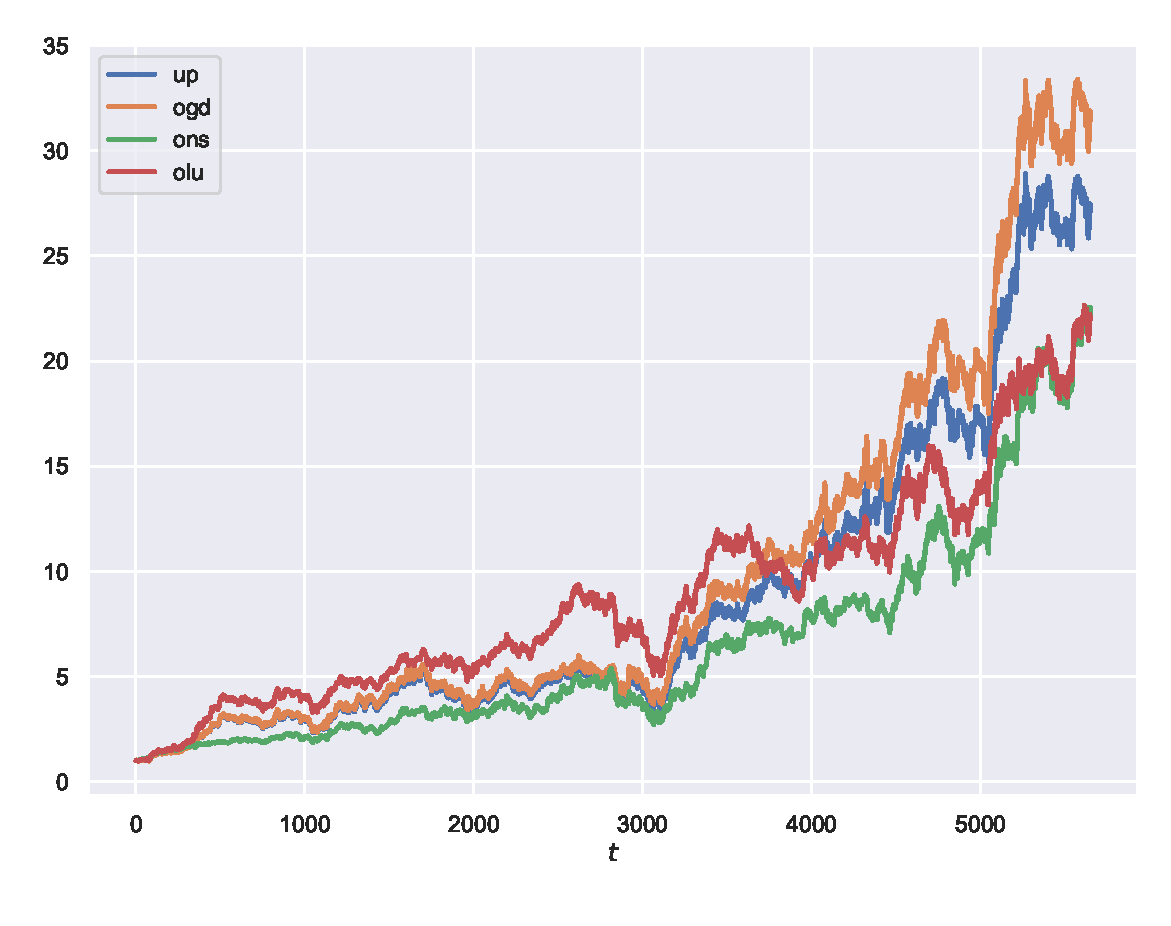
\includegraphics[width=0.48\textwidth,keepaspectratio]{img/fig_11.pdf}}
    \subfloat[\label{fig:ex2}]{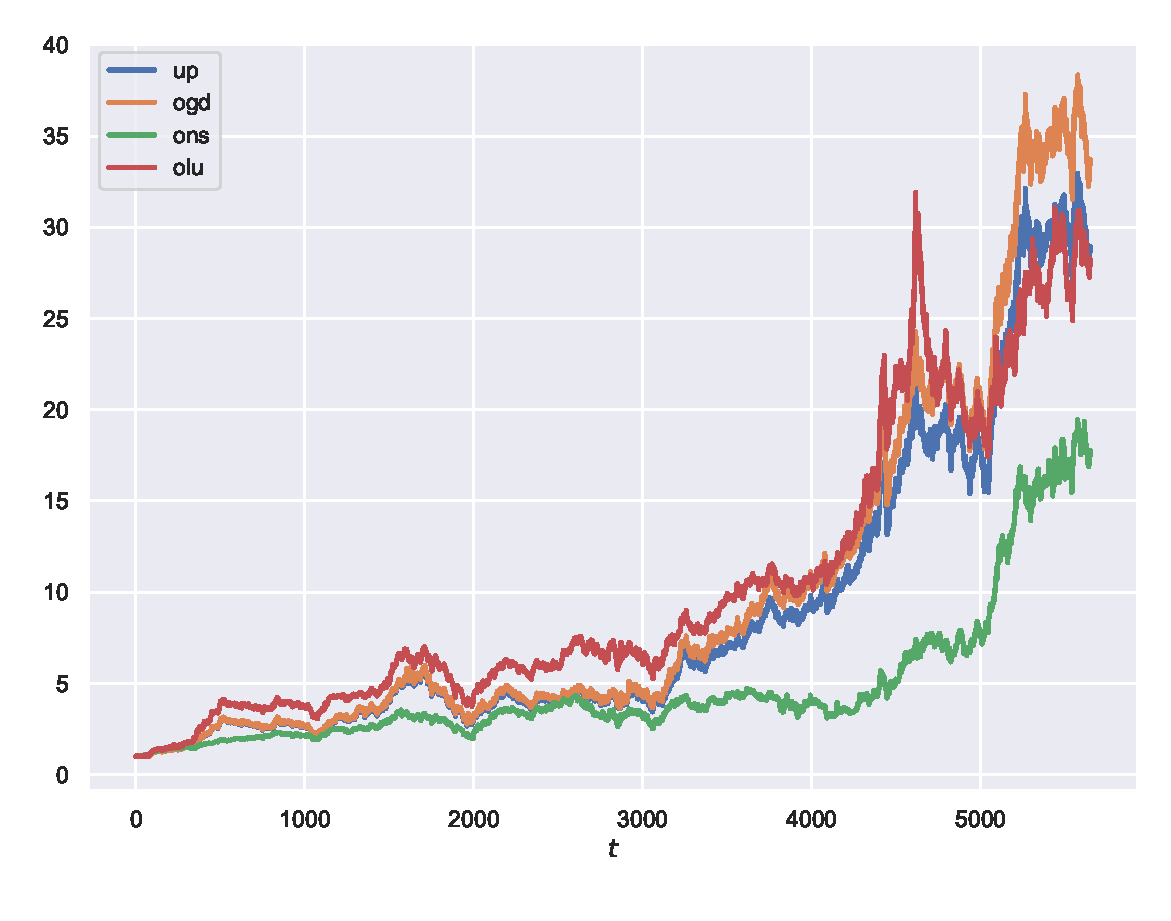
\includegraphics[width=0.48\textwidth,keepaspectratio]{img/fig_12.pdf}}
\caption{Wealth $W_T^C(\mathcal{A})$ on two runs of the NYSE(O) for $\gamma = 0$ (a), and $\gamma = 0.001$ (b).} \label{fig:algo_copmarison}
\end{figure}

Figure~\ref{fig:algo_copmarison} shows the evolution of the total wealth ${W}^C_t(\mathcal{A})$ of the different algorithms over the investment horizon in two specific runs, one without any cost ($\gamma = 0$) (Figure~\ref{fig:ex1}), and one with a transaction rate of $\gamma = 0.001$ (Figure~\ref{fig:ex2}).
In these two specific runs, OGD obtains a cumulative wealth larger than any other algorithm analyzed, suggesting that, in some settings, it might provide the best performance.
The results with $\gamma = 0$ suggest that OGD might be a viable solution even in the absence of costs.


\begin{figure}[ht!]
\centering
{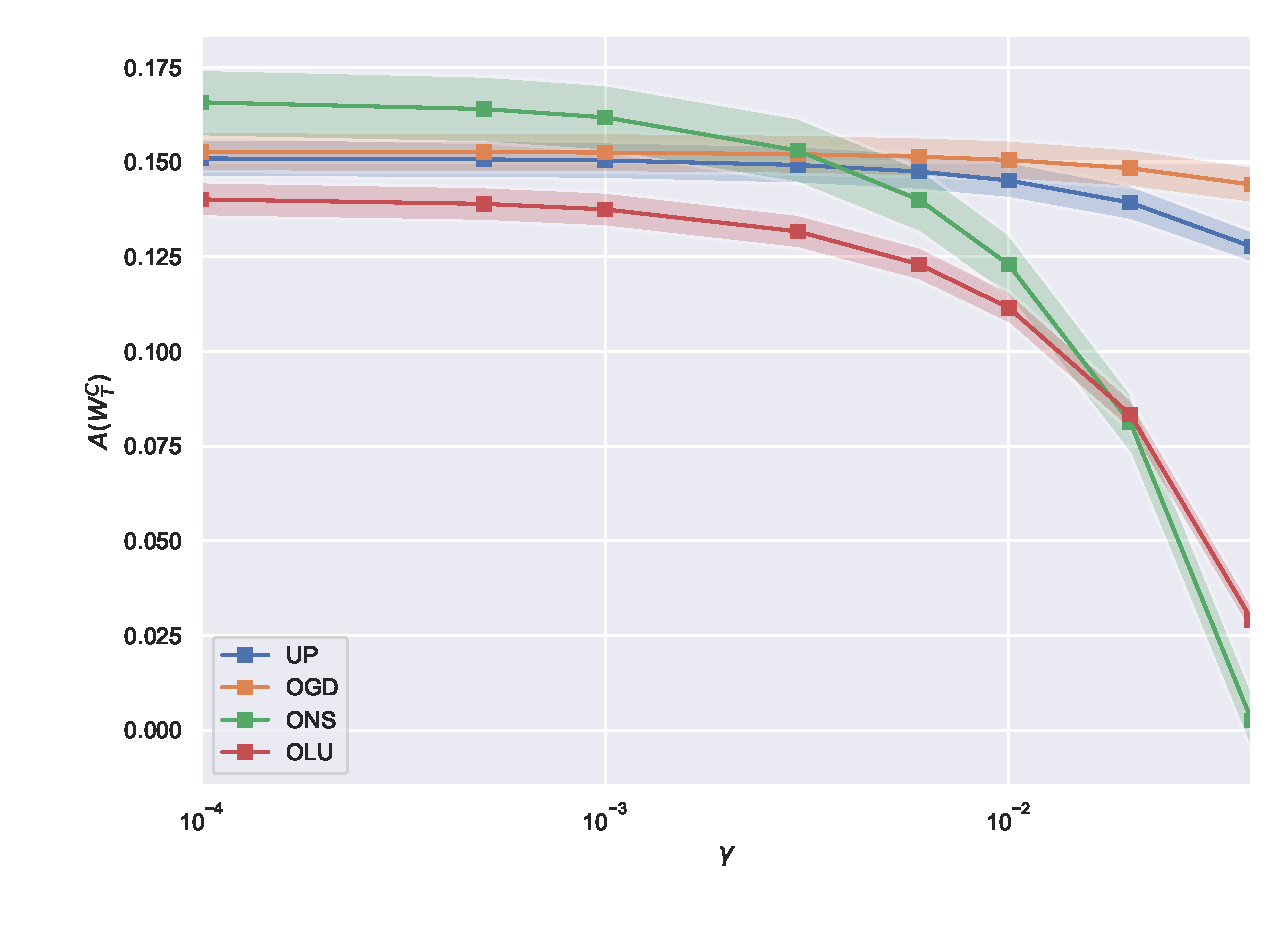
\includegraphics[width=0.70\textwidth,keepaspectratio]{img/fig_w_decay_l1.pdf}} 
\caption{Average APY computed on the wealth $W_T^C$ assuming the costs given by $C_T(\mathcal{A})$ for the NYSE(O) dataset.}
\label{fig:wealth_decay_l1}
\end{figure}

\begin{figure}[ht!]
\centering
{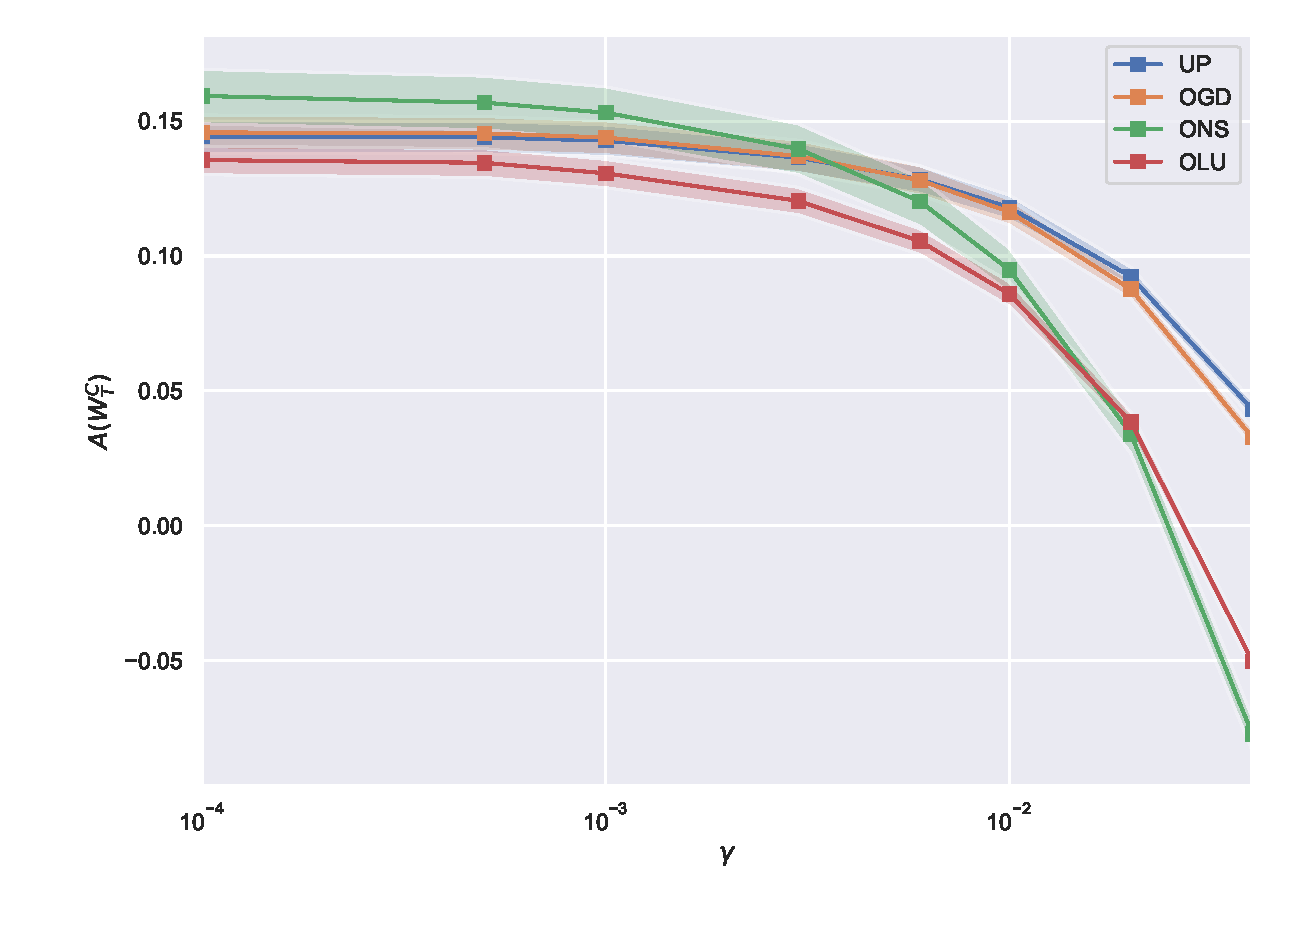
\includegraphics[width=0.70\textwidth,keepaspectratio]{img/fig_w_decay_true.pdf}} 
\caption{ Average APY computed on the wealth $\tilde{W}_T(\mathcal A)$ assuming the costs given by Equation~\eqref{eq:real_tc}, for the NYSE(O) dataset.}
\label{fig:wealth_decay_true}
\end{figure}

\begin{figure}[ht!]
\centering
{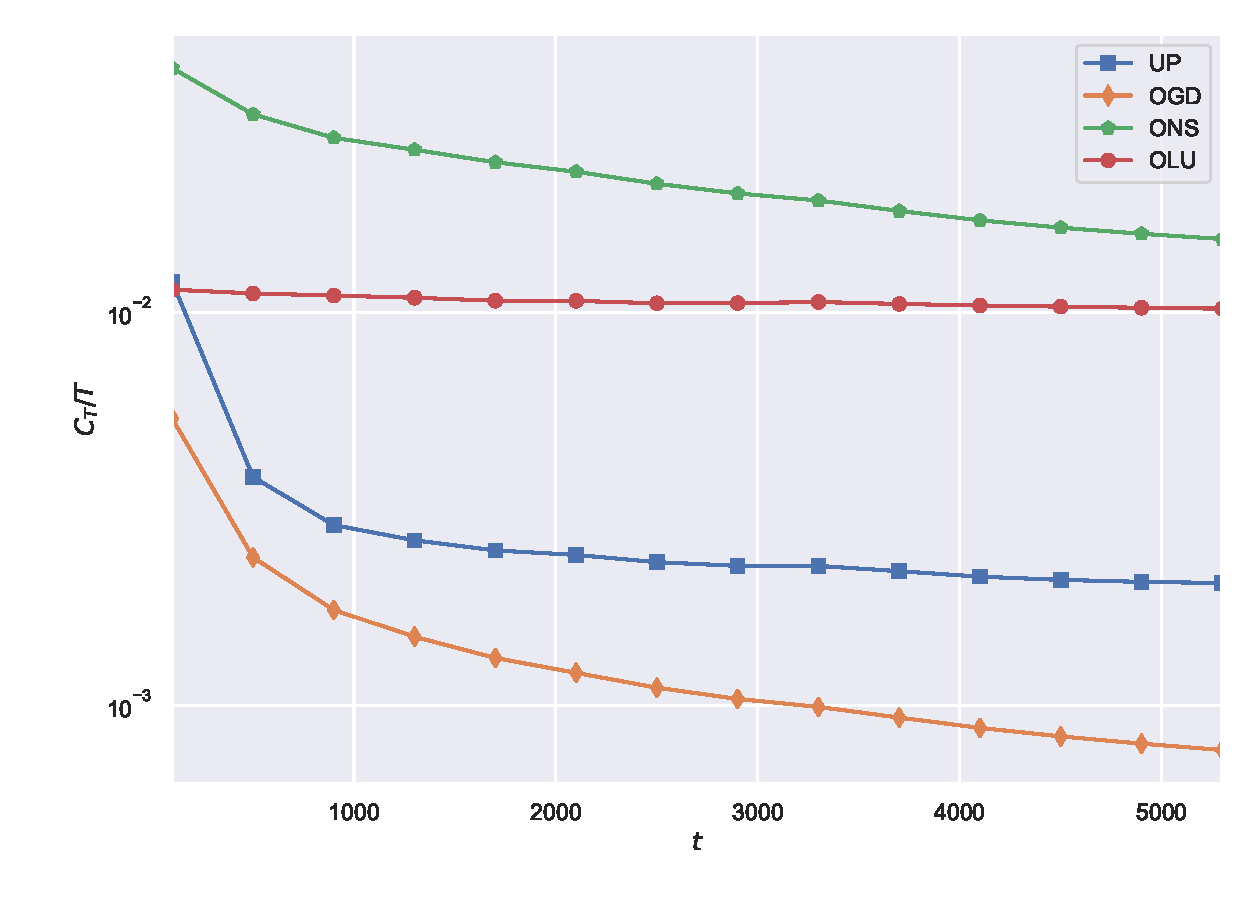
\includegraphics[width=0.70\textwidth,keepaspectratio]{img/fig_costs.pdf}}
\caption{Average costs $C_T(\mathcal{A})$ with $\gamma = 1$, for the NYSE(O) dataset.}
\label{fig:costs}
\end{figure}

In Figure~\ref{fig:wealth_decay_l1} we present the results for the average APY, with the corresponding confidence intervals.
In particular, with no transaction costs ($\gamma = 0$), all the analyzed algorithms give similar results.
In this setting, ONS is the algorithm with the largest APY.
As we increase the transaction rate $\gamma$, OGD gets the largest APY, while OLU and ONS seem to be penalized by large transaction costs.
Conversely, the fact that the APY decreases from $\approx 0.15$ to $\approx 0.14$ suggests that OGD is effective at minimizing the costs $C_T(\mathcal{A})$.

Figure~\ref{fig:wealth_decay_true} considers the wealth $\tilde{W}_T(\mathcal{A})$, \emph{i.e.}, the one defined in Equation~\eqref{eq:realwealth}.
We notice that, comparing these results with the ones obtained using $W_T^C$ (Figure~\ref{fig:wealth_decay_l1}), we have a smaller APY when $\gamma \gg 0$.
This suggests that, when applied to real-world cases, they might under-perform w.r.t.~what is expected from the theoretical results. 
In terms of $\tilde{W}_T(\mathcal{A})$, UP seems to perform slightly better than OGD, but the difference is not statistically significant for $\gamma < 0.04$.
ONS and OLU provide negative profits ($A(\tilde{W}_T) < 0$) for large values of transaction costs, \emph{e.g.}, for $\gamma = 0.04$ the APY becomes negative and, thus, the accumulated wealth is completely canceled out by the transaction costs.
From Figure~\ref{fig:wealth_decay_true} we would be inclined to choose ONS for $\gamma \leq 0.003$, and OGD for $\gamma \geq 0.003$.

Figure~\ref{fig:costs} shows the averaged cost per round $C_t(\mathcal{A})/t$ and the corresponding confidence intervals, with $\gamma = 1$ (the value of $\gamma$ has been chosen to easily interpret how the regret on the costs behaves over time).
OGD is the algorithm that provides the lowest cost per round, which strengthens the claim of this work that OGD keeps transaction costs low.
The costs per round for OLU are approximately linear, as expected from the theory (see Section~\ref{sec:OLU}).
Conversely, the results for ONS, while not having any theoretical guarantee on $C_T(\mathcal{A})/T$, suggest that it has a cost per round of order $\mathcal{O}(\sqrt{T})$, but with a larger constant than OGD.
Finally, the costs of UP decrease slower than those of ONS and OGD.

\subsection{Results on the TSE and SP500 dataset}

\begin{figure}[ht!]
\centering
{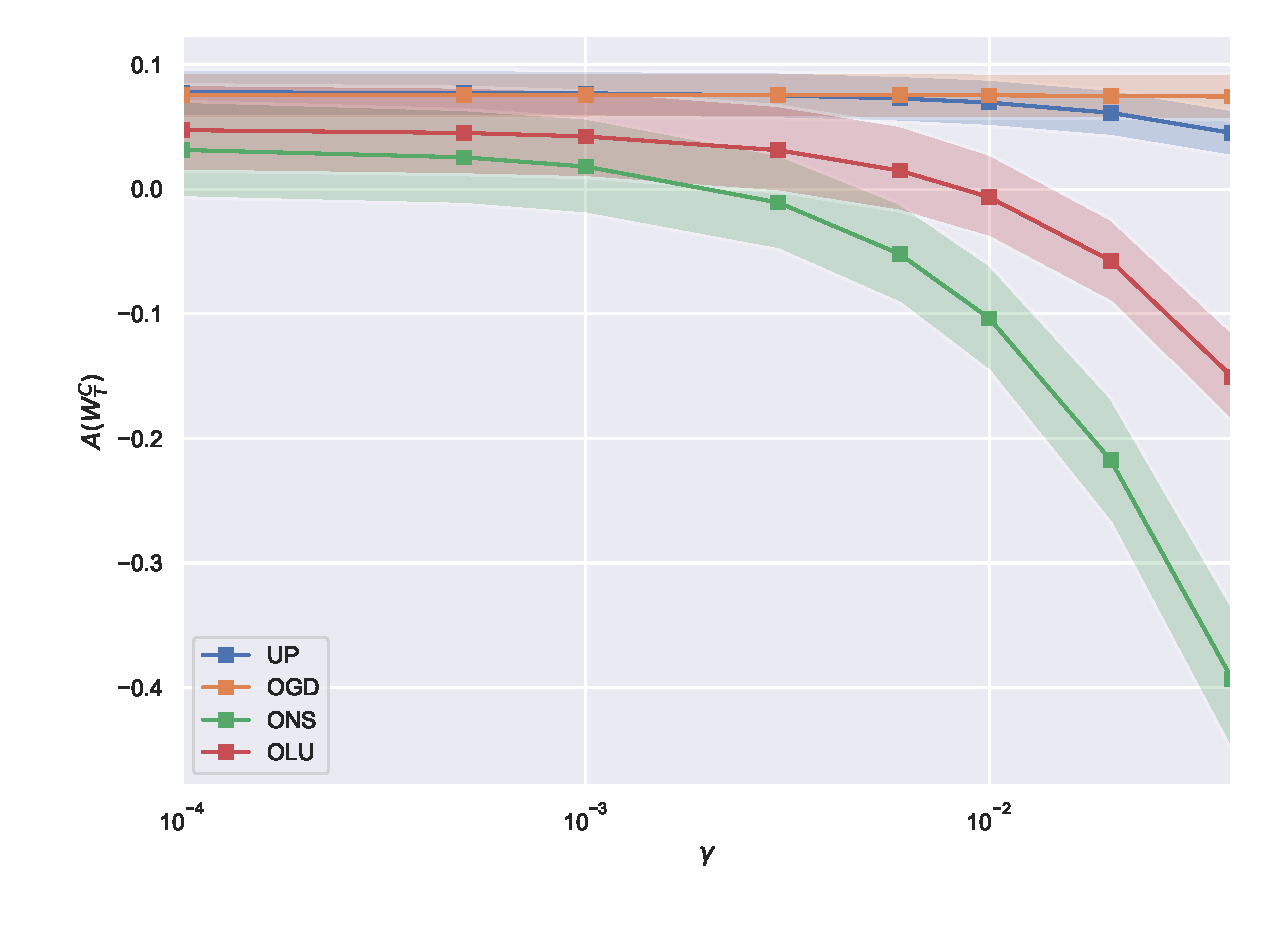
\includegraphics[width=0.70\textwidth,keepaspectratio]{img/fig_w_decay_l1_tse.pdf}} 
\caption{Average APY computed on the wealth $W_T^C$ assuming the costs given by $C_T(\mathcal{A})$ for the TSE dataset.}
\label{fig:wealth_decay_l1_tse}
\end{figure}

\begin{figure}[ht!]
\centering
{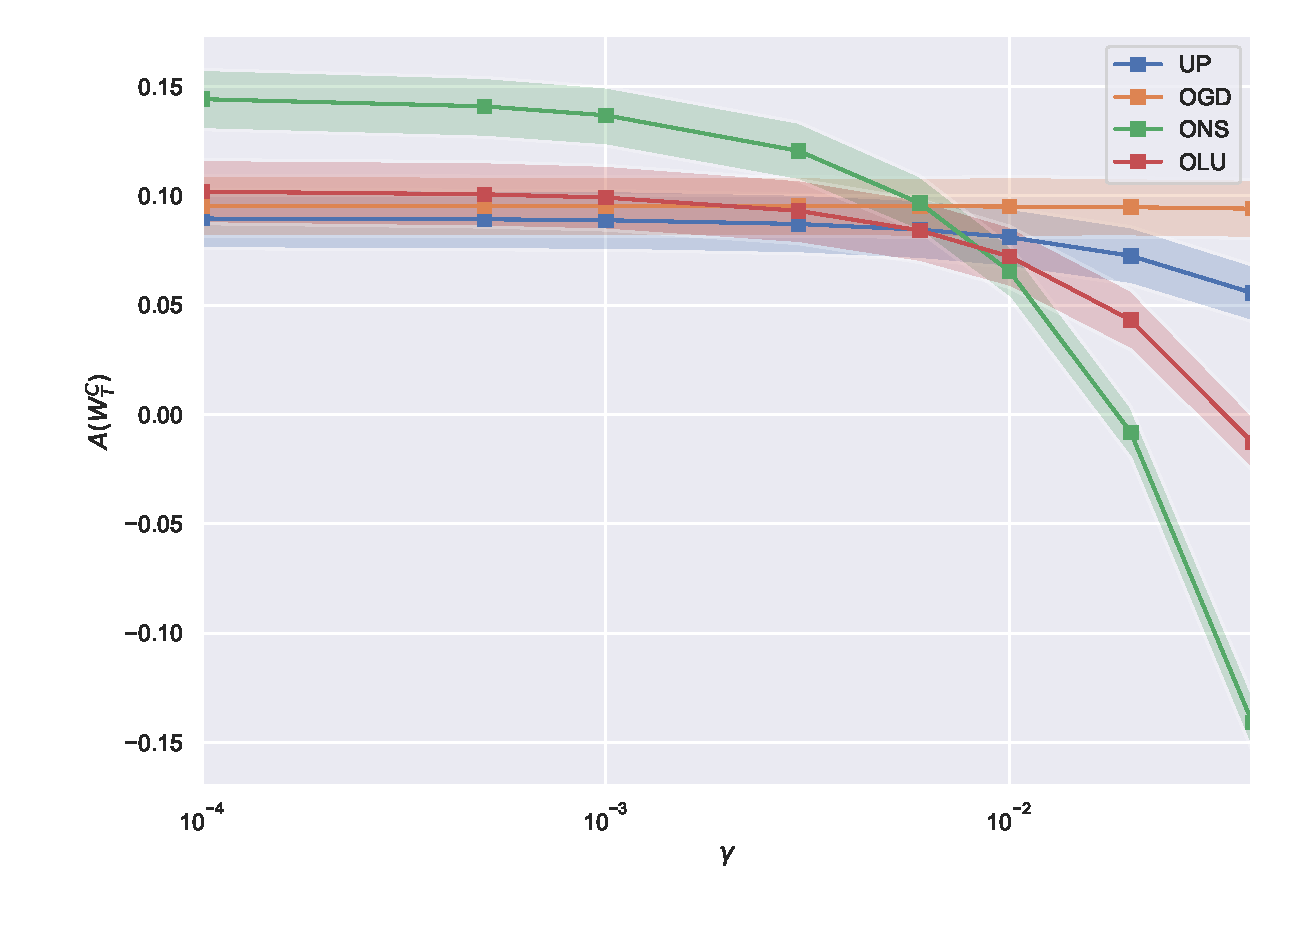
\includegraphics[width=0.70\textwidth,keepaspectratio]{img/fig_w_decay_l1_sp500.pdf}} 
\caption{Average APY computed on the wealth $W_T^C$ assuming the costs given by $C_T(\mathcal{A})$ for the SP500 dataset.}
\label{fig:wealth_decay_l1_sp500}
\end{figure}

In Figure \ref{fig:wealth_decay_l1_tse} and \ref{fig:wealth_decay_l1_sp500} we present the results obtained on the TSE and SP500 datasets respectively, using the same approach we used for the NYSE(O) dataset.  The results obtained are in line with the one presented with the NYSE(O) dataset, \emph{i.e.}, the OGD algorithm performs better than the others for transaction rate greater than $0.003$, while it presents similar performance, in terms of APY, for smaller values of the transaction rate. Notably, in the SP500 dataset, ONS outperforms the other algorithms for small transaction rate $\gamma$, while in the TSE dataset, it is out-performed by the other algorithms, even for small values of the transaction rate $\gamma$.

\section{Results on the Custom Dataset}

For the experiments carried out in this section, we collected a new dataset to test further the algorithms.

\begin{table}[ht!]\centering
\begin{tabular}{ |c||c|c| }
 \hline
 \multicolumn{3}{|c|}{Custom Data (03/29/2019 - 03/29/2020)} \\
 \hline
 Ticker & Description & Market Category\\
 \hline
 SPY & SPDR S\&P 500 ETF Trust (SPY)  & Equity\\
 BNDX &  Vanguard Bond Index Fund ETF & Fixed Income\\
 DAX & Global X DAX Germany ETF & Equity\\
 VIX & CBOE Volatility Index & Derivatives\\
 \hline
\end{tabular}
\caption{Detailed description of the custom dataset.}\label{tab:dataset_custom}
\end{table}

Table \ref{tab:dataset_custom} gives a description of the tailored dataset. We used data for one year (from April 2019 to April 2020), including the period of December 2019 - March 2020 that shows a global decline in the global financial markets. We included two Equity indices (SPY and DAX) as a proxy for the USA markets and European markets, then we included a Bond index (BNDX) and a volatility index (VIX) that simulate a Variance Swap, that allows investor to profit from volatility in the markets \cite{bossu2006introduction}.

We are well aware that a back-testing procedure not rigid enough can lead to over-fitting and biased results, which is an important problem in the financial literature (\cite{bailey2016probability}, \cite{harvey2015backtesting}).
Nonetheless, we found interesting to present these results, as these not only confirm the findings of the previous section, but also give insight on the inner workings of the algorithms. 

To set the parameters of ONS and OLU for the experiments performed on this dataset we used as a validation the first $1/4$ of the dataset (corresponding approximately to the first $3$ months of the dataset), performed  grid search algorithm and picked the parameters with the highest wealth $W_T$ on the validation set. The results of the grid search are presented in Figure \ref{fig:grid}. For the OGD algorithm we set the parameter $K$ to minimize the bound according to Theorem~\ref{thm:total_regret}.

\begin{figure}[ht!]
    \centering
    \subfloat[\label{fig:grdid_ONS}]{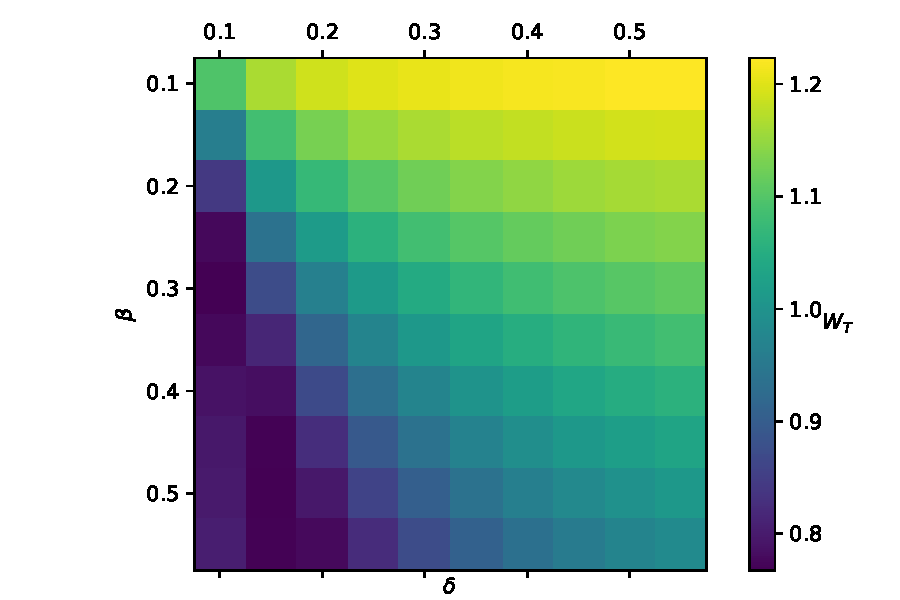
\includegraphics[width=0.48\textwidth,keepaspectratio]{img/grid_ONS.pdf}}
    \subfloat[\label{fig:grid_OLU}]{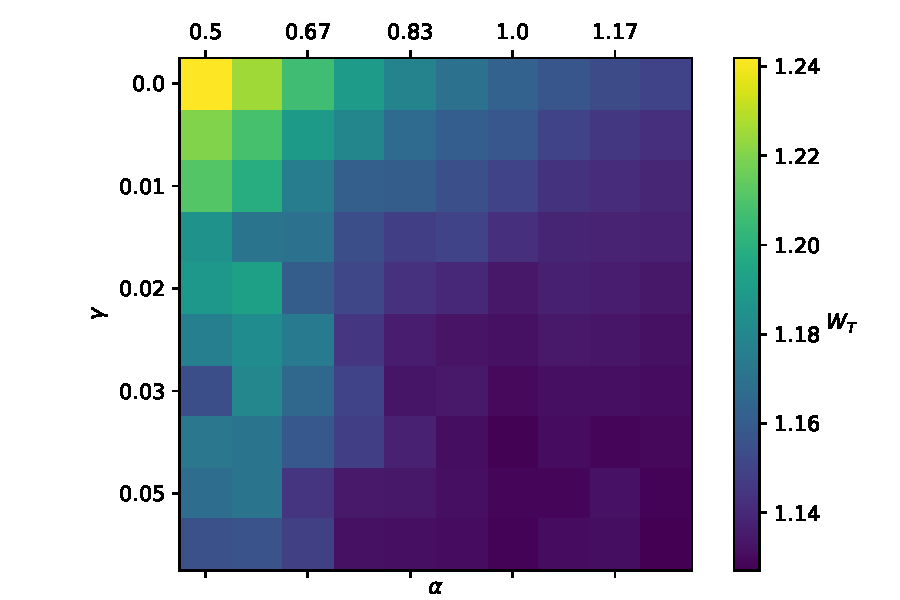
\includegraphics[width=0.48\textwidth,keepaspectratio]{img/grid_OLU.pdf}}
\caption{Grid search for the parameters of ONS (a) and OLU (b) on the validation set of the custom dataset.} \label{fig:grid}
\end{figure}

Figure \ref{fig:wealth_custom} shows the results for the algorithms run on the custom dataset. The transaction rate was set to $\gamma=0.001$ for all the algorithms. The reason why UP and OGD outperform the other two algorithms in this dataset, is the fact that they kept a larger portion of their allocation in the VIX index throughout the investment period. This lead to larger gains in the last two months. On the other hand ONS and OLU had nearly none of the VIX index in their allocations towards the end of the period, because it was performing poorly during the previous months. This lead to great losses in the last months of the trading period, due to the decrease of the other assets. 

In Figure \ref{fig:costs_custom} we show the dependency of the wealth achieved by algorithms to the transaction rate parameter $\gamma$ for the run on this dataset. We see how OGD shows a near constant wealth in relation to the transaction costs parameter $\gamma$, while UP only has a mild decline in wealth for large value of $\gamma$. Conversely, we see how ONS and OLU have a rapid decline in wealth w.r.t. the transaction rate $\gamma$.

\begin{figure}[ht!]
\centering
{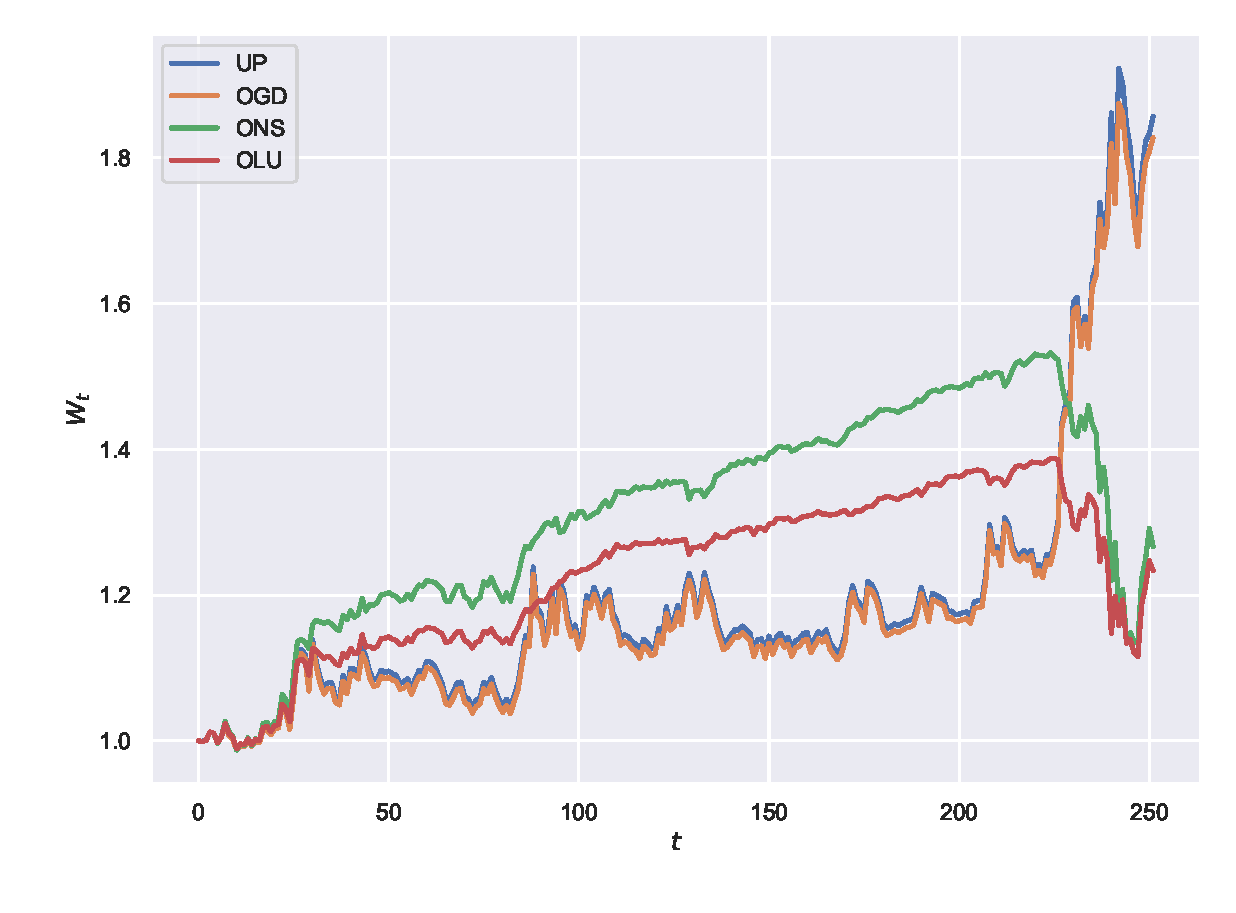
\includegraphics[width=0.70\textwidth,keepaspectratio]{img/new_experiemnts_1920.pdf}} 
\caption{Wealth $\tilde W_t$ achieved on the custom dataset described in Table \ref{tab:dataset_custom}, with $\gamma=0.001$.}
\label{fig:wealth_custom}
\end{figure}

\begin{figure}[ht!]
\centering
{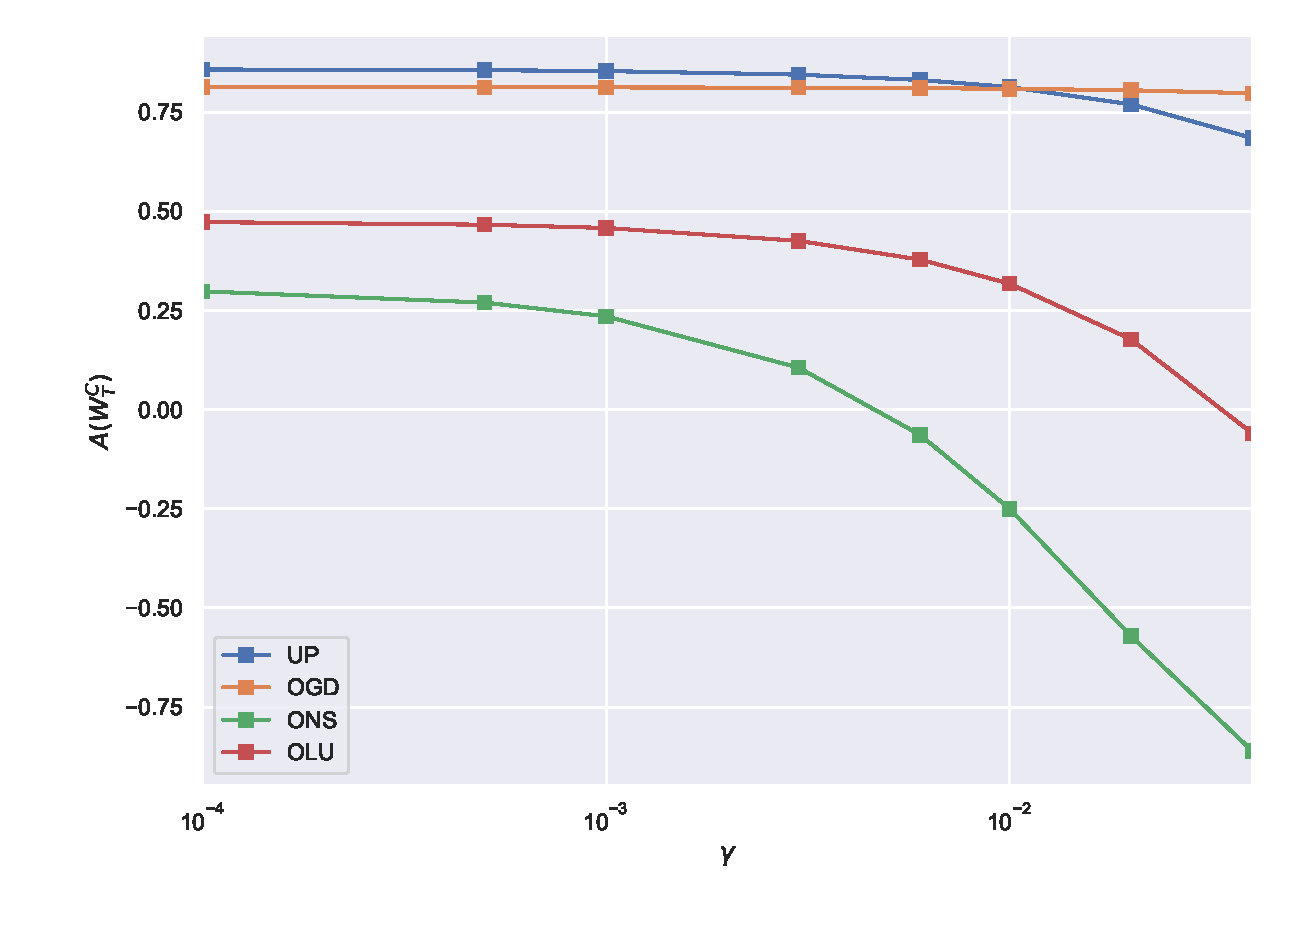
\includegraphics[width=0.70\textwidth,keepaspectratio]{img/new_experiemnts_1920_costs.pdf}} 
\caption{APY computed on the wealth $W_T^C(\mathcal A)$, assuming costs given by $C_T(\mathcal A)$ for the custom dataset.}
\label{fig:costs_custom}
\end{figure}

\chapter{Conclusions}\label{ch:conclusions}

Automated trading systems are becoming more and more central in the modern financial landscape \cite{treleaven2013algorithmic}. We explored an orthogonal approach to classical portfolio optimization methods that relies on concept of game theory and information theory. Since the most important properties of this methods are their strong theoretical guarantees on the wealth achieved by the algorithms, we extended the theoretical framework to include transaction costs and to recover the analytical guarantees under this, more realistic, framework.

Indeed, the focus of this thesis is to bound analytically transaction costs in the Online Portfolio Optimization problem.
We achieved this result by adapting, for the first time, to this context an algorithm from the field of Online Convex Optimization: the \emph{Online Gradient Descent}.
At first, we showed that the OGD has a total regret of the order of $\mathcal{O}(\sqrt{T})$, and a per-step computational complexity of $\Theta(N)$.
Then we showed that the other algorithms available in literature that provides theoretical guarantees in this context relies on unrealistic assumptions (OLU).
Finally, we compared the empirical performance of OGD with state-of-the-art algorithms on real datasets, and provided insights into the settings in which it is likely to provide larger cumulative wealth.

\section{Future Development}
Future developments of this work would be twofold.
Firstly we think that it would be possible to extend the transaction cost bound to a wider class of algorithms, \emph{e.g.}, the ones derived from Online Mirror Descent (OMD), in particular by exploiting the mirror interpretation of the OMD algorithm that relies on the concept of Fenchel conjugate, described in Section \ref{sec:mirror_version}.
On the other hand, even if the OGD already keeps the transaction costs at a pace, a possible extension would include costs as an explicit term in the objective function, \emph{i.e.}, develop cost-aware algorithms which still provide strong theoretical results.

Moreover, it would be interesting to extend the transaction costs model to include other kind of impediments encountered in a practical trading environment, such as liquidity constraints and market impact.


\cleardoublepage
\cleardoublepage

% ---- Bibliography ----
% \addcontentsline{toc}{chapter}{Bibliography}
% \bibliographystyle{plain}
\bibliographystyle{apalike}
\bibliography{bibl_thesis}

\appendix

%\pagestyle{fancy} 
%\fancyfoot{}                                               
%\renewcommand{\chaptermark}[1]{\markboth{\appendixname\ \thechapter.\ #1}{}} 
%\renewcommand{\sectionmark}[1]{\markright{\thesection.\ #1}}         
%\fancyhead[LE,RO]{\bfseries\thepage}    
%                                        
%\fancyhead[RE]{\bfseries\leftmark}    
%\fancyhead[LO]{\bfseries\rightmark}     
%\renewcommand{\headrulewidth}{0.3pt} 

%\include{appendices/appendixA}
\end{document}
